% a**************************************************************************************************************
% A Classic Thesis Style
% An Homage to The Elements of Typographic Style
%
% Copyright (C) 2018 André Miede and Ivo Pletikosić
%
% If you like the style then I would appreciate a postcard. My address
% can be found in the file ClassicThesis.pdf. A collection of the
% postcards I received so far is available online at
% http://postcards.miede.de
%
% License:
% This program is free software; you can redistribute it and/or modify
% it under the terms of the GNU General Public License as published by
% the Free Software Foundation; either version 2 of the License, or
% (at your option) any later version.
%
% This program is distributed in the hope that it will be useful,
% but WITHOUT ANY WARRANTY; without even the implied warranty of
% MERCHANTABILITY or FITNESS FOR A PARTICULAR PURPOSE.  See the
% GNU General Public License for more details.
%
% You should have received a copy of the GNU General Public License
% along with this program; see the file COPYING.  If not, write to
% the Free Software Foundation, Inc., 59 Temple Place - Suite 330,
% Boston, MA 02111-1307, USA.
%
% PLEASE SEE ALSO THE AUTHORS' NOTE REGARDING THIS LICENSE
% IN THE DOCUMENTATION (ClassicThesis.pdf --> Chapter 1 / Chapter01.tex)
% **************************************************************************************************************
\RequirePackage{silence} % :-\
    \WarningFilter{scrreprt}{Usage of package `titlesec'}
    %\WarningFilter{scrreprt}{Activating an ugly workaround}
    \WarningFilter{titlesec}{Non standard sectioning command detected}
\documentclass[ twoside,openright,titlepage,numbers=noenddot,%1headlines,
                headinclude,footinclude,cleardoublepage=empty,abstract=on,
                BCOR=5mm,paper=a4,fontsize=11pt,table,usenames,dvipsnames
                ]{scrreprt}

%********************************************************************
% Note: Make all your adjustments in here
%*******************************************************
% ****************************************************************************************************
% classicthesis-config.tex
% formerly known as loadpackages.sty, classicthesis-ldpkg.sty, and classicthesis-preamble.sty
% Use it at the beginning of your ClassicThesis.tex, or as a LaTeX Preamble
% in your ClassicThesis.{tex,lyx} with % ****************************************************************************************************
% classicthesis-config.tex
% formerly known as loadpackages.sty, classicthesis-ldpkg.sty, and classicthesis-preamble.sty
% Use it at the beginning of your ClassicThesis.tex, or as a LaTeX Preamble
% in your ClassicThesis.{tex,lyx} with % ****************************************************************************************************
% classicthesis-config.tex
% formerly known as loadpackages.sty, classicthesis-ldpkg.sty, and classicthesis-preamble.sty
% Use it at the beginning of your ClassicThesis.tex, or as a LaTeX Preamble
% in your ClassicThesis.{tex,lyx} with \input{classicthesis-config}
% ****************************************************************************************************
% If you like the classicthesis, then I would appreciate a postcard.
% My address can be found in the file ClassicThesis.pdf. A collection
% of the postcards I received so far is available online at
% http://postcards.miede.de
% ****************************************************************************************************


% ****************************************************************************************************
% 0. Set the encoding of your files. UTF-8 is the only sensible encoding nowadays. If you can't read
% äöüßáéçèê∂åëæƒÏ€ then change the encoding setting in your editor, not the line below. If your editor
% does not support utf8 use another editor!
% ****************************************************************************************************
\PassOptionsToPackage{utf8}{inputenc}
  \usepackage{inputenc}

\PassOptionsToPackage{T1}{fontenc} % T2A for cyrillics
  \usepackage{fontenc}


% ****************************************************************************************************
% 1. Configure classicthesis for your needs here, e.g., remove "drafting" below
% in order to deactivate the time-stamp on the pages
% (see ClassicThesis.pdf for more information):
% ****************************************************************************************************
\PassOptionsToPackage{
  drafting=true,    % print version information on the bottom of the pages
  tocaligned=false, % the left column of the toc will be aligned (no indentation)
  dottedtoc=false,  % page numbers in ToC flushed right
  eulerchapternumbers=true, % use AMS Euler for chapter font (otherwise Palatino)
  linedheaders=false,       % chaper headers will have line above and beneath
  floatperchapter=true,     % numbering per chapter for all floats (i.e., Figure 1.1)
  eulermath=false,  % use awesome Euler fonts for mathematical formulae (only with pdfLaTeX)
  beramono=true,    % toggle a nice monospaced font (w/ bold)
  palatino=true,    % deactivate standard font for loading another one, see the last section at the end of this file for suggestions
  style=classicthesis % classicthesis, arsclassica
}{classicthesis}


% ****************************************************************************************************
% 2. Personal data and user ad-hoc commands (insert your own data here)
% ****************************************************************************************************
\newcommand{\myTitle}{Linguaggi e programmazione orientata agli oggetti\xspace}
\newcommand{\mySubtitle}{Appunti\xspace}
\newcommand{\myDegree}{\xspace}
\newcommand{\myName}{Riccardo Cereghino\xspace}
\newcommand{\myProf}{Put name here\xspace}
\newcommand{\myOtherProf}{Put name here\xspace}
\newcommand{\mySupervisor}{Put name here\xspace}
\newcommand{\myFaculty}{Informatica\xspace}
\newcommand{\myDepartment}{DIBRIS\xspace}
\newcommand{\myUni}{Università di Genova\xspace}
\newcommand{\myLocation}{Genova\xspace}
\newcommand{\myTime}{Settembre 2019\xspace}
\newcommand{\myVersion}{\classicthesis}

% ********************************************************************
% Setup, finetuning, and useful commands
% ********************************************************************
\providecommand{\mLyX}{L\kern-.1667em\lower.25em\hbox{Y}\kern-.125emX\@}
\newcommand{\ie}{i.\,e.}
\newcommand{\Ie}{I.\,e.}
\newcommand{\eg}{e.\,g.}
\newcommand{\Eg}{E.\,g.}
% ****************************************************************************************************


% ****************************************************************************************************
% 3. Loading some handy packages
% ****************************************************************************************************
% ********************************************************************
% Packages with options that might require adjustments
% ********************************************************************
\PassOptionsToPackage{american, italian}{babel} % change this to your language(s), main language last
% Spanish languages need extra options in order to work with this template
%\PassOptionsToPackage{spanish,es-lcroman}{babel}
    \usepackage{babel}

\usepackage{csquotes}
\PassOptionsToPackage{%
  %backend=biber,bibencoding=utf8, %instead of bibtex
  backend=bibtex8,bibencoding=ascii,%
  language=auto,%
  style=numeric-comp,%
  %style=authoryear-comp, % Author 1999, 2010
  %bibstyle=authoryear,dashed=false, % dashed: substitute rep. author with ---
  sorting=nyt, % name, year, title
  maxbibnames=10, % default: 3, et al.
  %backref=true,%
  natbib=true % natbib compatibility mode (\citep and \citet still work)
}{biblatex}
    \usepackage{biblatex}

\PassOptionsToPackage{fleqn}{amsmath}       % math environments and more by the AMS
  \usepackage{amsmath}

% ********************************************************************
% General useful packages
% ********************************************************************
\usepackage{graphicx} %
\usepackage{scrhack} % fix warnings when using KOMA with listings package
\usepackage{xspace} % to get the spacing after macros right
\PassOptionsToPackage{printonlyused,smaller}{acronym}
  \usepackage{acronym} % nice macros for handling all acronyms in the thesis
  %\renewcommand{\bflabel}[1]{{#1}\hfill} % fix the list of acronyms --> no longer working
  %\renewcommand*{\acsfont}[1]{\textsc{#1}}
  %\renewcommand*{\aclabelfont}[1]{\acsfont{#1}}
  %\def\bflabel#1{{#1\hfill}}
  \def\bflabel#1{{\acsfont{#1}\hfill}}
  \def\aclabelfont#1{\acsfont{#1}}
% ****************************************************************************************************
%\usepackage{pgfplots} % External TikZ/PGF support (thanks to Andreas Nautsch)
%\usetikzlibrary{external}
%\tikzexternalize[mode=list and make, prefix=ext-tikz/]
% ****************************************************************************************************


% ****************************************************************************************************
% 4. Setup floats: tables, (sub)figures, and captions
% ****************************************************************************************************
\usepackage{tabularx} % better tables
  \setlength{\extrarowheight}{3pt} % increase table row height
\newcommand{\tableheadline}[1]{\multicolumn{1}{l}{\spacedlowsmallcaps{#1}}}
\newcommand{\myfloatalign}{\centering} % to be used with each float for alignment
\usepackage{subfig}
% ****************************************************************************************************


% ****************************************************************************************************
% 5. Setup code listings
% ****************************************************************************************************
\usepackage{listings}
%\lstset{emph={trueIndex,root},emphstyle=\color{BlueViolet}}%\underbar} % for special keywords
\lstset{language=Java,
  morekeywords={PassOptionsToPackage,selectlanguage},
  keywordstyle=\color{RoyalBlue},%\bfseries,
  basicstyle=\small\ttfamily,
  identifierstyle=\color{NavyBlue},
  commentstyle=\color{Green}\ttfamily,
  stringstyle=\rmfamily,
  numbers=none,%left,%
  numberstyle=\scriptsize,%\tiny
  stepnumber=5,
  numbersep=8pt,
  showstringspaces=false,
  breaklines=true,
  frameround=ftff,
  frame=single,
  belowcaptionskip=.75\baselineskip,
  frame=L
}
% ****************************************************************************************************




% ****************************************************************************************************
% 6. Last calls before the bar closes
% ****************************************************************************************************
\usepackage{amssymb}
\usepackage{ntheorem}

\let\numberset\mathbb
\newcommand{\N}{\numberset{N}}
\newcommand{\Z}{\numberset{Z}}
\newcommand{\Q}{\numberset{Q}}
\newcommand{\R}{\numberset{R}}
\newcommand{\C}{\numberset{C}}
\newcommand{\U}{\numberset{U}}
\newcommand{\I}{\numberset{I}}
\newcommand{\PP}{\numberset{P}}
\newcommand{\CC}{\complement}
\newcommand{\dom}{\text{dom }}
\newcommand{\im}{\text{Im }}
\newcommand{\foi}{\text{f.i.}}
\newcommand{\e}{\mathrm{e}}
\newcommand{\cc}{\mathcal{C}}
\newcommand{\dd}{\mathrm{d}}

\usepackage{float}
\usepackage{wrapfig}

\usepackage{import}
\usepackage{xifthen}
\usepackage{pdfpages}
\usepackage{transparent}

\newcommand{\incfig}[1]{%
    \def\svgwidth{0.25\columnwidth}
    \import{./figures/}{#1.pdf_tex}
}
\pdfsuppresswarningpagegroup=1
\usepackage{tikz}
% ********************************************************************
% Her Majesty herself
% ********************************************************************
\usepackage{classicthesis}


% ********************************************************************
% Fine-tune hyperreferences (hyperref should be called last)
% ********************************************************************
\hypersetup{%
  %draft, % hyperref's draft mode, for printing see below
  colorlinks=true, linktocpage=true, pdfstartpage=3, pdfstartview=FitV,%
  % uncomment the following line if you want to have black links (e.g., for printing)
  %colorlinks=false, linktocpage=false, pdfstartpage=3, pdfstartview=FitV, pdfborder={0 0 0},%
  breaklinks=true, pageanchor=true,%
  pdfpagemode=UseNone, %
  % pdfpagemode=UseOutlines,%
  plainpages=false, bookmarksnumbered, bookmarksopen=true, bookmarksopenlevel=1,%
  hypertexnames=true, pdfhighlight=/O,%nesting=true,%frenchlinks,%
  urlcolor=CTurl, linkcolor=CTlink, citecolor=CTcitation, %pagecolor=RoyalBlue,%
  %urlcolor=Black, linkcolor=Black, citecolor=Black, %pagecolor=Black,%
  pdftitle={\myTitle},%
  pdfauthor={\textcopyright\ \myName, \myUni, \myFaculty},%
  pdfsubject={},%
  pdfkeywords={},%
  pdfcreator={pdfLaTeX},%
  pdfproducer={LaTeX with hyperref and classicthesis}%
}


% ********************************************************************
% Setup autoreferences (hyperref and babel)
% ********************************************************************
% There are some issues regarding autorefnames
% http://www.tex.ac.uk/cgi-bin/texfaq2html?label=latexwords
% you have to redefine the macros for the
% language you use, e.g., american, ngerman
% (as chosen when loading babel/AtBeginDocument)
% ********************************************************************
\makeatletter
\@ifpackageloaded{babel}%
  {%
    \addto\extrasamerican{%
      \renewcommand*{\figureautorefname}{Figure}%
      \renewcommand*{\tableautorefname}{Table}%
      \renewcommand*{\partautorefname}{Part}%
      \renewcommand*{\chapterautorefname}{Chapter}%
      \renewcommand*{\sectionautorefname}{Section}%
      \renewcommand*{\subsectionautorefname}{Section}%
      \renewcommand*{\subsubsectionautorefname}{Section}%
    }%
    \addto\extrasngerman{%
      \renewcommand*{\paragraphautorefname}{Absatz}%
      \renewcommand*{\subparagraphautorefname}{Unterabsatz}%
      \renewcommand*{\footnoteautorefname}{Fu\"snote}%
      \renewcommand*{\FancyVerbLineautorefname}{Zeile}%
      \renewcommand*{\theoremautorefname}{Theorem}%
      \renewcommand*{\appendixautorefname}{Anhang}%
      \renewcommand*{\equationautorefname}{Gleichung}%
      \renewcommand*{\itemautorefname}{Punkt}%
    }%
      % Fix to getting autorefs for subfigures right (thanks to Belinda Vogt for changing the definition)
      \providecommand{\subfigureautorefname}{\figureautorefname}%
    }{\relax}
\makeatother


% ********************************************************************
% Development Stuff
% ********************************************************************
\listfiles
%\PassOptionsToPackage{l2tabu,orthodox,abort}{nag}
%  \usepackage{nag}
%\PassOptionsToPackage{warning, all}{onlyamsmath}
%  \usepackage{onlyamsmath}


% ****************************************************************************************************
% 7. Further adjustments (experimental)
% ****************************************************************************************************
% ********************************************************************
% Changing the text area
% ********************************************************************
%\areaset[current]{312pt}{761pt} % 686 (factor 2.2) + 33 head + 42 head \the\footskip
%\setlength{\marginparwidth}{7em}%
%\setlength{\marginparsep}{2em}%

% ********************************************************************
% Using different fonts
% ********************************************************************
%\usepackage[oldstylenums]{kpfonts} % oldstyle notextcomp
% \usepackage[osf]{libertine}
%\usepackage[light,condensed,math]{iwona}
%\renewcommand{\sfdefault}{iwona}
%\usepackage{lmodern} % <-- no osf support :-(
%\usepackage{cfr-lm} %
%\usepackage[urw-garamond]{mathdesign} <-- no osf support :-(
%\usepackage[default,osfigures]{opensans} % scale=0.95
%\usepackage[sfdefault]{FiraSans}
% \usepackage[opticals,mathlf]{MinionPro} % onlytext
% ********************************************************************
%\usepackage[largesc,osf]{newpxtext}
%\linespread{1.05} % a bit more for Palatino
% Used to fix these:
% https://bitbucket.org/amiede/classicthesis/issues/139/italics-in-pallatino-capitals-chapter
% https://bitbucket.org/amiede/classicthesis/issues/45/problema-testatine-su-classicthesis-style
% ********************************************************************
% ****************************************************************************************************

% ****************************************************************************************************
% If you like the classicthesis, then I would appreciate a postcard.
% My address can be found in the file ClassicThesis.pdf. A collection
% of the postcards I received so far is available online at
% http://postcards.miede.de
% ****************************************************************************************************


% ****************************************************************************************************
% 0. Set the encoding of your files. UTF-8 is the only sensible encoding nowadays. If you can't read
% äöüßáéçèê∂åëæƒÏ€ then change the encoding setting in your editor, not the line below. If your editor
% does not support utf8 use another editor!
% ****************************************************************************************************
\PassOptionsToPackage{utf8}{inputenc}
  \usepackage{inputenc}

\PassOptionsToPackage{T1}{fontenc} % T2A for cyrillics
  \usepackage{fontenc}


% ****************************************************************************************************
% 1. Configure classicthesis for your needs here, e.g., remove "drafting" below
% in order to deactivate the time-stamp on the pages
% (see ClassicThesis.pdf for more information):
% ****************************************************************************************************
\PassOptionsToPackage{
  drafting=true,    % print version information on the bottom of the pages
  tocaligned=false, % the left column of the toc will be aligned (no indentation)
  dottedtoc=false,  % page numbers in ToC flushed right
  eulerchapternumbers=true, % use AMS Euler for chapter font (otherwise Palatino)
  linedheaders=false,       % chaper headers will have line above and beneath
  floatperchapter=true,     % numbering per chapter for all floats (i.e., Figure 1.1)
  eulermath=false,  % use awesome Euler fonts for mathematical formulae (only with pdfLaTeX)
  beramono=true,    % toggle a nice monospaced font (w/ bold)
  palatino=true,    % deactivate standard font for loading another one, see the last section at the end of this file for suggestions
  style=classicthesis % classicthesis, arsclassica
}{classicthesis}


% ****************************************************************************************************
% 2. Personal data and user ad-hoc commands (insert your own data here)
% ****************************************************************************************************
\newcommand{\myTitle}{Linguaggi e programmazione orientata agli oggetti\xspace}
\newcommand{\mySubtitle}{Appunti\xspace}
\newcommand{\myDegree}{\xspace}
\newcommand{\myName}{Riccardo Cereghino\xspace}
\newcommand{\myProf}{Put name here\xspace}
\newcommand{\myOtherProf}{Put name here\xspace}
\newcommand{\mySupervisor}{Put name here\xspace}
\newcommand{\myFaculty}{Informatica\xspace}
\newcommand{\myDepartment}{DIBRIS\xspace}
\newcommand{\myUni}{Università di Genova\xspace}
\newcommand{\myLocation}{Genova\xspace}
\newcommand{\myTime}{Settembre 2019\xspace}
\newcommand{\myVersion}{\classicthesis}

% ********************************************************************
% Setup, finetuning, and useful commands
% ********************************************************************
\providecommand{\mLyX}{L\kern-.1667em\lower.25em\hbox{Y}\kern-.125emX\@}
\newcommand{\ie}{i.\,e.}
\newcommand{\Ie}{I.\,e.}
\newcommand{\eg}{e.\,g.}
\newcommand{\Eg}{E.\,g.}
% ****************************************************************************************************


% ****************************************************************************************************
% 3. Loading some handy packages
% ****************************************************************************************************
% ********************************************************************
% Packages with options that might require adjustments
% ********************************************************************
\PassOptionsToPackage{american, italian}{babel} % change this to your language(s), main language last
% Spanish languages need extra options in order to work with this template
%\PassOptionsToPackage{spanish,es-lcroman}{babel}
    \usepackage{babel}

\usepackage{csquotes}
\PassOptionsToPackage{%
  %backend=biber,bibencoding=utf8, %instead of bibtex
  backend=bibtex8,bibencoding=ascii,%
  language=auto,%
  style=numeric-comp,%
  %style=authoryear-comp, % Author 1999, 2010
  %bibstyle=authoryear,dashed=false, % dashed: substitute rep. author with ---
  sorting=nyt, % name, year, title
  maxbibnames=10, % default: 3, et al.
  %backref=true,%
  natbib=true % natbib compatibility mode (\citep and \citet still work)
}{biblatex}
    \usepackage{biblatex}

\PassOptionsToPackage{fleqn}{amsmath}       % math environments and more by the AMS
  \usepackage{amsmath}

% ********************************************************************
% General useful packages
% ********************************************************************
\usepackage{graphicx} %
\usepackage{scrhack} % fix warnings when using KOMA with listings package
\usepackage{xspace} % to get the spacing after macros right
\PassOptionsToPackage{printonlyused,smaller}{acronym}
  \usepackage{acronym} % nice macros for handling all acronyms in the thesis
  %\renewcommand{\bflabel}[1]{{#1}\hfill} % fix the list of acronyms --> no longer working
  %\renewcommand*{\acsfont}[1]{\textsc{#1}}
  %\renewcommand*{\aclabelfont}[1]{\acsfont{#1}}
  %\def\bflabel#1{{#1\hfill}}
  \def\bflabel#1{{\acsfont{#1}\hfill}}
  \def\aclabelfont#1{\acsfont{#1}}
% ****************************************************************************************************
%\usepackage{pgfplots} % External TikZ/PGF support (thanks to Andreas Nautsch)
%\usetikzlibrary{external}
%\tikzexternalize[mode=list and make, prefix=ext-tikz/]
% ****************************************************************************************************


% ****************************************************************************************************
% 4. Setup floats: tables, (sub)figures, and captions
% ****************************************************************************************************
\usepackage{tabularx} % better tables
  \setlength{\extrarowheight}{3pt} % increase table row height
\newcommand{\tableheadline}[1]{\multicolumn{1}{l}{\spacedlowsmallcaps{#1}}}
\newcommand{\myfloatalign}{\centering} % to be used with each float for alignment
\usepackage{subfig}
% ****************************************************************************************************


% ****************************************************************************************************
% 5. Setup code listings
% ****************************************************************************************************
\usepackage{listings}
%\lstset{emph={trueIndex,root},emphstyle=\color{BlueViolet}}%\underbar} % for special keywords
\lstset{language=Java,
  morekeywords={PassOptionsToPackage,selectlanguage},
  keywordstyle=\color{RoyalBlue},%\bfseries,
  basicstyle=\small\ttfamily,
  identifierstyle=\color{NavyBlue},
  commentstyle=\color{Green}\ttfamily,
  stringstyle=\rmfamily,
  numbers=none,%left,%
  numberstyle=\scriptsize,%\tiny
  stepnumber=5,
  numbersep=8pt,
  showstringspaces=false,
  breaklines=true,
  frameround=ftff,
  frame=single,
  belowcaptionskip=.75\baselineskip,
  frame=L
}
% ****************************************************************************************************




% ****************************************************************************************************
% 6. Last calls before the bar closes
% ****************************************************************************************************
\usepackage{amssymb}
\usepackage{ntheorem}

\let\numberset\mathbb
\newcommand{\N}{\numberset{N}}
\newcommand{\Z}{\numberset{Z}}
\newcommand{\Q}{\numberset{Q}}
\newcommand{\R}{\numberset{R}}
\newcommand{\C}{\numberset{C}}
\newcommand{\U}{\numberset{U}}
\newcommand{\I}{\numberset{I}}
\newcommand{\PP}{\numberset{P}}
\newcommand{\CC}{\complement}
\newcommand{\dom}{\text{dom }}
\newcommand{\im}{\text{Im }}
\newcommand{\foi}{\text{f.i.}}
\newcommand{\e}{\mathrm{e}}
\newcommand{\cc}{\mathcal{C}}
\newcommand{\dd}{\mathrm{d}}

\usepackage{float}
\usepackage{wrapfig}

\usepackage{import}
\usepackage{xifthen}
\usepackage{pdfpages}
\usepackage{transparent}

\newcommand{\incfig}[1]{%
    \def\svgwidth{0.25\columnwidth}
    \import{./figures/}{#1.pdf_tex}
}
\pdfsuppresswarningpagegroup=1
\usepackage{tikz}
% ********************************************************************
% Her Majesty herself
% ********************************************************************
\usepackage{classicthesis}


% ********************************************************************
% Fine-tune hyperreferences (hyperref should be called last)
% ********************************************************************
\hypersetup{%
  %draft, % hyperref's draft mode, for printing see below
  colorlinks=true, linktocpage=true, pdfstartpage=3, pdfstartview=FitV,%
  % uncomment the following line if you want to have black links (e.g., for printing)
  %colorlinks=false, linktocpage=false, pdfstartpage=3, pdfstartview=FitV, pdfborder={0 0 0},%
  breaklinks=true, pageanchor=true,%
  pdfpagemode=UseNone, %
  % pdfpagemode=UseOutlines,%
  plainpages=false, bookmarksnumbered, bookmarksopen=true, bookmarksopenlevel=1,%
  hypertexnames=true, pdfhighlight=/O,%nesting=true,%frenchlinks,%
  urlcolor=CTurl, linkcolor=CTlink, citecolor=CTcitation, %pagecolor=RoyalBlue,%
  %urlcolor=Black, linkcolor=Black, citecolor=Black, %pagecolor=Black,%
  pdftitle={\myTitle},%
  pdfauthor={\textcopyright\ \myName, \myUni, \myFaculty},%
  pdfsubject={},%
  pdfkeywords={},%
  pdfcreator={pdfLaTeX},%
  pdfproducer={LaTeX with hyperref and classicthesis}%
}


% ********************************************************************
% Setup autoreferences (hyperref and babel)
% ********************************************************************
% There are some issues regarding autorefnames
% http://www.tex.ac.uk/cgi-bin/texfaq2html?label=latexwords
% you have to redefine the macros for the
% language you use, e.g., american, ngerman
% (as chosen when loading babel/AtBeginDocument)
% ********************************************************************
\makeatletter
\@ifpackageloaded{babel}%
  {%
    \addto\extrasamerican{%
      \renewcommand*{\figureautorefname}{Figure}%
      \renewcommand*{\tableautorefname}{Table}%
      \renewcommand*{\partautorefname}{Part}%
      \renewcommand*{\chapterautorefname}{Chapter}%
      \renewcommand*{\sectionautorefname}{Section}%
      \renewcommand*{\subsectionautorefname}{Section}%
      \renewcommand*{\subsubsectionautorefname}{Section}%
    }%
    \addto\extrasngerman{%
      \renewcommand*{\paragraphautorefname}{Absatz}%
      \renewcommand*{\subparagraphautorefname}{Unterabsatz}%
      \renewcommand*{\footnoteautorefname}{Fu\"snote}%
      \renewcommand*{\FancyVerbLineautorefname}{Zeile}%
      \renewcommand*{\theoremautorefname}{Theorem}%
      \renewcommand*{\appendixautorefname}{Anhang}%
      \renewcommand*{\equationautorefname}{Gleichung}%
      \renewcommand*{\itemautorefname}{Punkt}%
    }%
      % Fix to getting autorefs for subfigures right (thanks to Belinda Vogt for changing the definition)
      \providecommand{\subfigureautorefname}{\figureautorefname}%
    }{\relax}
\makeatother


% ********************************************************************
% Development Stuff
% ********************************************************************
\listfiles
%\PassOptionsToPackage{l2tabu,orthodox,abort}{nag}
%  \usepackage{nag}
%\PassOptionsToPackage{warning, all}{onlyamsmath}
%  \usepackage{onlyamsmath}


% ****************************************************************************************************
% 7. Further adjustments (experimental)
% ****************************************************************************************************
% ********************************************************************
% Changing the text area
% ********************************************************************
%\areaset[current]{312pt}{761pt} % 686 (factor 2.2) + 33 head + 42 head \the\footskip
%\setlength{\marginparwidth}{7em}%
%\setlength{\marginparsep}{2em}%

% ********************************************************************
% Using different fonts
% ********************************************************************
%\usepackage[oldstylenums]{kpfonts} % oldstyle notextcomp
% \usepackage[osf]{libertine}
%\usepackage[light,condensed,math]{iwona}
%\renewcommand{\sfdefault}{iwona}
%\usepackage{lmodern} % <-- no osf support :-(
%\usepackage{cfr-lm} %
%\usepackage[urw-garamond]{mathdesign} <-- no osf support :-(
%\usepackage[default,osfigures]{opensans} % scale=0.95
%\usepackage[sfdefault]{FiraSans}
% \usepackage[opticals,mathlf]{MinionPro} % onlytext
% ********************************************************************
%\usepackage[largesc,osf]{newpxtext}
%\linespread{1.05} % a bit more for Palatino
% Used to fix these:
% https://bitbucket.org/amiede/classicthesis/issues/139/italics-in-pallatino-capitals-chapter
% https://bitbucket.org/amiede/classicthesis/issues/45/problema-testatine-su-classicthesis-style
% ********************************************************************
% ****************************************************************************************************

% ****************************************************************************************************
% If you like the classicthesis, then I would appreciate a postcard.
% My address can be found in the file ClassicThesis.pdf. A collection
% of the postcards I received so far is available online at
% http://postcards.miede.de
% ****************************************************************************************************


% ****************************************************************************************************
% 0. Set the encoding of your files. UTF-8 is the only sensible encoding nowadays. If you can't read
% äöüßáéçèê∂åëæƒÏ€ then change the encoding setting in your editor, not the line below. If your editor
% does not support utf8 use another editor!
% ****************************************************************************************************
\PassOptionsToPackage{utf8}{inputenc}
  \usepackage{inputenc}

\PassOptionsToPackage{T1}{fontenc} % T2A for cyrillics
  \usepackage{fontenc}


% ****************************************************************************************************
% 1. Configure classicthesis for your needs here, e.g., remove "drafting" below
% in order to deactivate the time-stamp on the pages
% (see ClassicThesis.pdf for more information):
% ****************************************************************************************************
\PassOptionsToPackage{
  drafting=true,    % print version information on the bottom of the pages
  tocaligned=false, % the left column of the toc will be aligned (no indentation)
  dottedtoc=false,  % page numbers in ToC flushed right
  eulerchapternumbers=true, % use AMS Euler for chapter font (otherwise Palatino)
  linedheaders=false,       % chaper headers will have line above and beneath
  floatperchapter=true,     % numbering per chapter for all floats (i.e., Figure 1.1)
  eulermath=false,  % use awesome Euler fonts for mathematical formulae (only with pdfLaTeX)
  beramono=true,    % toggle a nice monospaced font (w/ bold)
  palatino=true,    % deactivate standard font for loading another one, see the last section at the end of this file for suggestions
  style=classicthesis % classicthesis, arsclassica
}{classicthesis}


% ****************************************************************************************************
% 2. Personal data and user ad-hoc commands (insert your own data here)
% ****************************************************************************************************
\newcommand{\myTitle}{Linguaggi e programmazione orientata agli oggetti\xspace}
\newcommand{\mySubtitle}{Appunti\xspace}
\newcommand{\myDegree}{\xspace}
\newcommand{\myName}{Riccardo Cereghino\xspace}
\newcommand{\myProf}{Put name here\xspace}
\newcommand{\myOtherProf}{Put name here\xspace}
\newcommand{\mySupervisor}{Put name here\xspace}
\newcommand{\myFaculty}{Informatica\xspace}
\newcommand{\myDepartment}{DIBRIS\xspace}
\newcommand{\myUni}{Università di Genova\xspace}
\newcommand{\myLocation}{Genova\xspace}
\newcommand{\myTime}{Settembre 2019\xspace}
\newcommand{\myVersion}{\classicthesis}

% ********************************************************************
% Setup, finetuning, and useful commands
% ********************************************************************
\providecommand{\mLyX}{L\kern-.1667em\lower.25em\hbox{Y}\kern-.125emX\@}
\newcommand{\ie}{i.\,e.}
\newcommand{\Ie}{I.\,e.}
\newcommand{\eg}{e.\,g.}
\newcommand{\Eg}{E.\,g.}
% ****************************************************************************************************


% ****************************************************************************************************
% 3. Loading some handy packages
% ****************************************************************************************************
% ********************************************************************
% Packages with options that might require adjustments
% ********************************************************************
\PassOptionsToPackage{american, italian}{babel} % change this to your language(s), main language last
% Spanish languages need extra options in order to work with this template
%\PassOptionsToPackage{spanish,es-lcroman}{babel}
    \usepackage{babel}

\usepackage{csquotes}
\PassOptionsToPackage{%
  %backend=biber,bibencoding=utf8, %instead of bibtex
  backend=bibtex8,bibencoding=ascii,%
  language=auto,%
  style=numeric-comp,%
  %style=authoryear-comp, % Author 1999, 2010
  %bibstyle=authoryear,dashed=false, % dashed: substitute rep. author with ---
  sorting=nyt, % name, year, title
  maxbibnames=10, % default: 3, et al.
  %backref=true,%
  natbib=true % natbib compatibility mode (\citep and \citet still work)
}{biblatex}
    \usepackage{biblatex}

\PassOptionsToPackage{fleqn}{amsmath}       % math environments and more by the AMS
  \usepackage{amsmath}

% ********************************************************************
% General useful packages
% ********************************************************************
\usepackage{graphicx} %
\usepackage{scrhack} % fix warnings when using KOMA with listings package
\usepackage{xspace} % to get the spacing after macros right
\PassOptionsToPackage{printonlyused,smaller}{acronym}
  \usepackage{acronym} % nice macros for handling all acronyms in the thesis
  %\renewcommand{\bflabel}[1]{{#1}\hfill} % fix the list of acronyms --> no longer working
  %\renewcommand*{\acsfont}[1]{\textsc{#1}}
  %\renewcommand*{\aclabelfont}[1]{\acsfont{#1}}
  %\def\bflabel#1{{#1\hfill}}
  \def\bflabel#1{{\acsfont{#1}\hfill}}
  \def\aclabelfont#1{\acsfont{#1}}
% ****************************************************************************************************
%\usepackage{pgfplots} % External TikZ/PGF support (thanks to Andreas Nautsch)
%\usetikzlibrary{external}
%\tikzexternalize[mode=list and make, prefix=ext-tikz/]
% ****************************************************************************************************


% ****************************************************************************************************
% 4. Setup floats: tables, (sub)figures, and captions
% ****************************************************************************************************
\usepackage{tabularx} % better tables
  \setlength{\extrarowheight}{3pt} % increase table row height
\newcommand{\tableheadline}[1]{\multicolumn{1}{l}{\spacedlowsmallcaps{#1}}}
\newcommand{\myfloatalign}{\centering} % to be used with each float for alignment
\usepackage{subfig}
% ****************************************************************************************************


% ****************************************************************************************************
% 5. Setup code listings
% ****************************************************************************************************
\usepackage{listings}
%\lstset{emph={trueIndex,root},emphstyle=\color{BlueViolet}}%\underbar} % for special keywords
\lstset{language=Java,
  morekeywords={PassOptionsToPackage,selectlanguage},
  keywordstyle=\color{RoyalBlue},%\bfseries,
  basicstyle=\small\ttfamily,
  identifierstyle=\color{NavyBlue},
  commentstyle=\color{Green}\ttfamily,
  stringstyle=\rmfamily,
  numbers=none,%left,%
  numberstyle=\scriptsize,%\tiny
  stepnumber=5,
  numbersep=8pt,
  showstringspaces=false,
  breaklines=true,
  frameround=ftff,
  frame=single,
  belowcaptionskip=.75\baselineskip,
  frame=L
}
% ****************************************************************************************************




% ****************************************************************************************************
% 6. Last calls before the bar closes
% ****************************************************************************************************
\usepackage{amssymb}
\usepackage{ntheorem}

\let\numberset\mathbb
\newcommand{\N}{\numberset{N}}
\newcommand{\Z}{\numberset{Z}}
\newcommand{\Q}{\numberset{Q}}
\newcommand{\R}{\numberset{R}}
\newcommand{\C}{\numberset{C}}
\newcommand{\U}{\numberset{U}}
\newcommand{\I}{\numberset{I}}
\newcommand{\PP}{\numberset{P}}
\newcommand{\CC}{\complement}
\newcommand{\dom}{\text{dom }}
\newcommand{\im}{\text{Im }}
\newcommand{\foi}{\text{f.i.}}
\newcommand{\e}{\mathrm{e}}
\newcommand{\cc}{\mathcal{C}}
\newcommand{\dd}{\mathrm{d}}

\usepackage{float}
\usepackage{wrapfig}

\usepackage{import}
\usepackage{xifthen}
\usepackage{pdfpages}
\usepackage{transparent}

\newcommand{\incfig}[1]{%
    \def\svgwidth{0.25\columnwidth}
    \import{./figures/}{#1.pdf_tex}
}
\pdfsuppresswarningpagegroup=1
\usepackage{tikz}
% ********************************************************************
% Her Majesty herself
% ********************************************************************
\usepackage{classicthesis}


% ********************************************************************
% Fine-tune hyperreferences (hyperref should be called last)
% ********************************************************************
\hypersetup{%
  %draft, % hyperref's draft mode, for printing see below
  colorlinks=true, linktocpage=true, pdfstartpage=3, pdfstartview=FitV,%
  % uncomment the following line if you want to have black links (e.g., for printing)
  %colorlinks=false, linktocpage=false, pdfstartpage=3, pdfstartview=FitV, pdfborder={0 0 0},%
  breaklinks=true, pageanchor=true,%
  pdfpagemode=UseNone, %
  % pdfpagemode=UseOutlines,%
  plainpages=false, bookmarksnumbered, bookmarksopen=true, bookmarksopenlevel=1,%
  hypertexnames=true, pdfhighlight=/O,%nesting=true,%frenchlinks,%
  urlcolor=CTurl, linkcolor=CTlink, citecolor=CTcitation, %pagecolor=RoyalBlue,%
  %urlcolor=Black, linkcolor=Black, citecolor=Black, %pagecolor=Black,%
  pdftitle={\myTitle},%
  pdfauthor={\textcopyright\ \myName, \myUni, \myFaculty},%
  pdfsubject={},%
  pdfkeywords={},%
  pdfcreator={pdfLaTeX},%
  pdfproducer={LaTeX with hyperref and classicthesis}%
}


% ********************************************************************
% Setup autoreferences (hyperref and babel)
% ********************************************************************
% There are some issues regarding autorefnames
% http://www.tex.ac.uk/cgi-bin/texfaq2html?label=latexwords
% you have to redefine the macros for the
% language you use, e.g., american, ngerman
% (as chosen when loading babel/AtBeginDocument)
% ********************************************************************
\makeatletter
\@ifpackageloaded{babel}%
  {%
    \addto\extrasamerican{%
      \renewcommand*{\figureautorefname}{Figure}%
      \renewcommand*{\tableautorefname}{Table}%
      \renewcommand*{\partautorefname}{Part}%
      \renewcommand*{\chapterautorefname}{Chapter}%
      \renewcommand*{\sectionautorefname}{Section}%
      \renewcommand*{\subsectionautorefname}{Section}%
      \renewcommand*{\subsubsectionautorefname}{Section}%
    }%
    \addto\extrasngerman{%
      \renewcommand*{\paragraphautorefname}{Absatz}%
      \renewcommand*{\subparagraphautorefname}{Unterabsatz}%
      \renewcommand*{\footnoteautorefname}{Fu\"snote}%
      \renewcommand*{\FancyVerbLineautorefname}{Zeile}%
      \renewcommand*{\theoremautorefname}{Theorem}%
      \renewcommand*{\appendixautorefname}{Anhang}%
      \renewcommand*{\equationautorefname}{Gleichung}%
      \renewcommand*{\itemautorefname}{Punkt}%
    }%
      % Fix to getting autorefs for subfigures right (thanks to Belinda Vogt for changing the definition)
      \providecommand{\subfigureautorefname}{\figureautorefname}%
    }{\relax}
\makeatother


% ********************************************************************
% Development Stuff
% ********************************************************************
\listfiles
%\PassOptionsToPackage{l2tabu,orthodox,abort}{nag}
%  \usepackage{nag}
%\PassOptionsToPackage{warning, all}{onlyamsmath}
%  \usepackage{onlyamsmath}


% ****************************************************************************************************
% 7. Further adjustments (experimental)
% ****************************************************************************************************
% ********************************************************************
% Changing the text area
% ********************************************************************
%\areaset[current]{312pt}{761pt} % 686 (factor 2.2) + 33 head + 42 head \the\footskip
%\setlength{\marginparwidth}{7em}%
%\setlength{\marginparsep}{2em}%

% ********************************************************************
% Using different fonts
% ********************************************************************
%\usepackage[oldstylenums]{kpfonts} % oldstyle notextcomp
% \usepackage[osf]{libertine}
%\usepackage[light,condensed,math]{iwona}
%\renewcommand{\sfdefault}{iwona}
%\usepackage{lmodern} % <-- no osf support :-(
%\usepackage{cfr-lm} %
%\usepackage[urw-garamond]{mathdesign} <-- no osf support :-(
%\usepackage[default,osfigures]{opensans} % scale=0.95
%\usepackage[sfdefault]{FiraSans}
% \usepackage[opticals,mathlf]{MinionPro} % onlytext
% ********************************************************************
%\usepackage[largesc,osf]{newpxtext}
%\linespread{1.05} % a bit more for Palatino
% Used to fix these:
% https://bitbucket.org/amiede/classicthesis/issues/139/italics-in-pallatino-capitals-chapter
% https://bitbucket.org/amiede/classicthesis/issues/45/problema-testatine-su-classicthesis-style
% ********************************************************************
% ****************************************************************************************************


%********************************************************************
% Bibliographies
%*******************************************************
%\addbibresource{Bibliography.bib}
%\addbibresource[label=ownpubs]{AMiede_Publications.bib}

%********************************************************************
% Hyphenation
%*******************************************************
%\hyphenation{put special hyphenation here}

% ********************************************************************
% GO!GO!GO! MOVE IT!
%*******************************************************
\begin{document}
\frenchspacing
\raggedbottom
\selectlanguage{italian} % american ngerman
%\renewcommand*{\bibname}{new name}
%\setbibpreamble{}
\pagenumbering{roman}
\pagestyle{plain}
\newtheorem{theorem}{Definizione}

%********************************************************************
% Frontmatter
%*******************************************************
%%*******************************************************
% Little Dirty Titlepage
%*******************************************************
\thispagestyle{empty}
%\pdfbookmark[1]{Titel}{title}
%*******************************************************
\begin{center}
    \spacedlowsmallcaps{\myName} \\ \medskip

    \begingroup
        \color{CTtitle}\spacedallcaps{\myTitle}
    \endgroup
\end{center}

%*******************************************************
% Titlepage
%*******************************************************
\begin{titlepage}
    %\pdfbookmark[1]{\myTitle}{titlepage}
    % if you want the titlepage to be centered, uncomment and fine-tune the line below (KOMA classes environment)
    \begin{addmargin}[-1cm]{-3cm}
    \begin{center}
        \large

        \hfill

        \vfill

        \begingroup
            \color{CTtitle}\spacedallcaps{\myTitle} \\ \bigskip
        \endgroup

        \spacedlowsmallcaps{\myName}

        \vfill

        
\includegraphics[width=6cm]{gfx/TFZsuperellipse_bw} \\ \medskip

        \mySubtitle \\ \medskip
        %\myDegree \\
        %\myDepartment \\
        %\myFaculty \\
        %\myUni \\ \bigskip

        \myTime\ -- \myVersion

        \vfill

    \end{center}
  \end{addmargin}
\end{titlepage}

%\thispagestyle{empty}

\hfill

\vfill

\noindent\myName: \textit{\myTitle,} \mySubtitle, %\myDegree,
\textcopyright\ \myTime

%\bigskip
%
%\noindent\spacedlowsmallcaps{Supervisors}: \\
%\myProf \\
%\myOtherProf \\
%\mySupervisor
%
%\medskip
%
%\noindent\spacedlowsmallcaps{Location}: \\
%\myLocation
%
%\medskip
%
%\noindent\spacedlowsmallcaps{Time Frame}: \\
%\myTime

%\cleardoublepage%*******************************************************
% Dedication
%*******************************************************
\thispagestyle{empty}
\phantomsection
\pdfbookmark[1]{Dedication}{Dedication}

\vspace*{3cm}

\begin{center}
    \emph{Ohana} means family. \\
    Family means nobody gets left behind, or forgotten. \\ \medskip
    --- Lilo \& Stitch
\end{center}

\medskip

\begin{center}
    Dedicated to the loving memory of Rudolf Miede. \\ \smallskip
    1939\,--\,2005
\end{center}

%\cleardoublepage\include{FrontBackmatter/Foreword}
%\cleardoublepage%*******************************************************
% Abstract
%*******************************************************
%\renewcommand{\abstractname}{Abstract}
\pdfbookmark[1]{Abstract}{Abstract}
% \addcontentsline{toc}{chapter}{\tocEntry{Abstract}}
\begingroup
\let\clearpage\relax
\let\cleardoublepage\relax
\let\cleardoublepage\relax

\chapter*{Abstract}
Short summary of the contents in English\dots a great guide by
Kent Beck how to write good abstracts can be found here:
\begin{center}
\url{https://plg.uwaterloo.ca/~migod/research/beckOOPSLA.html}
\end{center}

\vfill

\begin{otherlanguage}{ngerman}
\pdfbookmark[1]{Zusammenfassung}{Zusammenfassung}
\chapter*{Zusammenfassung}
Kurze Zusammenfassung des Inhaltes in deutscher Sprache\dots
\end{otherlanguage}

\endgroup

\vfill

%\cleardoublepage%*******************************************************
% Publications
%*******************************************************
\pdfbookmark[1]{Publications}{publications}
\chapter*{Publications}\graffito{This is just an early --~and currently ugly~-- test!}
This might come in handy for PhD theses: some ideas and figures have appeared previously in the following publications:

%\noindent Put your publications from the thesis here. The packages \texttt{multibib} or \texttt{bibtopic} etc. can be used to handle multiple different bibliographies in your document.

\begin{refsection}[ownpubs]
    \small
    \nocite{*} % is local to to the enclosing refsection
    \printbibliography[heading=none]
\end{refsection}

\emph{Attention}: This requires a separate run of \texttt{bibtex} for your \texttt{refsection}, \eg, \texttt{ClassicThesis1-blx} for this file. You might also use \texttt{biber} as the backend for \texttt{biblatex}. See also \url{http://tex.stackexchange.com/questions/128196/problem-with-refsection}.

%\cleardoublepage%*******************************************************
% Acknowledgments
%*******************************************************
\pdfbookmark[1]{Acknowledgments}{acknowledgments}

\begin{flushright}{\slshape
    We have seen that computer programming is an art, \\
    because it applies accumulated knowledge to the world, \\
    because it requires skill and ingenuity, and especially \\
    because it produces objects of beauty.} \\ \medskip
    --- \defcitealias{knuth:1974}{Donald E. Knuth}\citetalias{knuth:1974} \citep{knuth:1974}
\end{flushright}



\bigskip

\begingroup
\let\clearpage\relax
\let\cleardoublepage\relax
\let\cleardoublepage\relax
\chapter*{Acknowledgments}
Put your acknowledgments here.

Many thanks to everybody who already sent me a postcard!

Regarding the typography and other help, many thanks go to Marco
Kuhlmann, Philipp Lehman, Lothar Schlesier, Jim Young, Lorenzo
Pantieri and Enrico Gregorio\footnote{Members of GuIT (Gruppo
Italiano Utilizzatori di \TeX\ e \LaTeX )}, J\"org Sommer,
Joachim K\"ostler, Daniel Gottschlag, Denis Aydin, Paride
Legovini, Steffen Prochnow, Nicolas Repp, Hinrich Harms,
Roland Winkler, Jörg Weber, Henri Menke, Claus Lahiri,
Clemens Niederberger, Stefano Bragaglia, Jörn Hees,
Scott Lowe, Dave Howcroft, Jos\'e M. Alcaide, David Carlisle,
Ulrike Fischer, Hugues de Lassus, Csaba Hajdu, Dave Howcroft, 
and the whole \LaTeX-community for support, ideas and
some great software.

\bigskip

\noindent\emph{Regarding \mLyX}: The \mLyX\ port was intially done by
\emph{Nicholas Mariette} in March 2009 and continued by
\emph{Ivo Pletikosi\'c} in 2011. Thank you very much for your
work and for the contributions to the original style.


\endgroup

\cleardoublepage%*******************************************************
% Table of Contents
%*******************************************************
\pagestyle{scrheadings}
%\phantomsection
\pdfbookmark[1]{\contentsname}{tableofcontents}
\setcounter{tocdepth}{2} % <-- 2 includes up to subsections in the ToC
\setcounter{secnumdepth}{3} % <-- 3 numbers up to subsubsections
\manualmark
\markboth{\spacedlowsmallcaps{\contentsname}}{\spacedlowsmallcaps{\contentsname}}
\tableofcontents
\automark[section]{chapter}
\renewcommand{\chaptermark}[1]{\markboth{\spacedlowsmallcaps{#1}}{\spacedlowsmallcaps{#1}}}
\renewcommand{\sectionmark}[1]{\markright{\textsc{\thesection}\enspace\spacedlowsmallcaps{#1}}}
%*******************************************************
% List of Figures and of the Tables
%*******************************************************
\clearpage
% \pagestyle{empty} % Uncomment this line if your lists should not have any headlines with section name and page number
\begingroup
    \let\clearpage\relax
    \let\cleardoublepage\relax
    %*******************************************************
    % List of Figures
    %*******************************************************
    %\phantomsection
    %\addcontentsline{toc}{chapter}{\listfigurename}
    \pdfbookmark[1]{\listfigurename}{lof}
    \listoffigures

    \vspace{8ex}

    %*******************************************************
    % List of Tables
    %*******************************************************
    %\phantomsection
    %\addcontentsline{toc}{chapter}{\listtablename}
    %\pdfbookmark[1]{\listtablename}{lot}
    %\listoftables

    %\vspace{8ex}
    % \newpage

    %*******************************************************
    % List of Listings
    %*******************************************************
    %\phantomsection
    %\addcontentsline{toc}{chapter}{\lstlistlistingname}
    \pdfbookmark[1]{\lstlistlistingname}{lol}
    \lstlistoflistings

    \vspace{8ex}

    %*******************************************************
    % Acronyms
    %*******************************************************
    %\phantomsection
    %\pdfbookmark[1]{Acronyms}{acronyms}
    %\markboth{\spacedlowsmallcaps{Acronyms}}{\spacedlowsmallcaps{Acronyms}}
    %\chapter*{Acronyms}
    %\begin{acronym}[UMLX]
        %\acro{DRY}{Don't Repeat Yourself}
        %\acro{API}{Application Programming Interface}
        %\acro{UML}{Unified Modeling Language}
    %\end{acronym}

\endgroup

%********************************************************************
% Mainmatter
%*******************************************************
\cleardoublepage
\pagestyle{scrheadings}
\pagenumbering{arabic}
%\setcounter{page}{90}
% use \cleardoublepage here to avoid problems with pdfbookmark
%\cleardoublepage
\chapter{Introduzione agli elementi di un linguaggio di programmazione}\label{ch:elementi}
I motivi della creazione ed utilizzo di un linguaggio di programmazione di
alto livello sono:
di fornire una descrizione precisa, ovvero una specifica formale;
offrire un interpretazione tramite interprete da compilare.

Le caratteristiche principali che categorizzano i linguaggi di
programmazione sono la sintassi e la semantica, la quale può essere
statica o dinamica.

\section{Linguaggi staticamente tipati}
Nei linguaggi tipizzati staticamente il \emph{tipo} di variabile viene
stabilito nel codice sorgente, per cui si rende necessario che:

\begin{itemize}
  \item gli operatori e le assegnazioni devono essere usati coerentemente
    con il \emph{tipo} dichiarato;
  \item le variabili siano usate consistentemente rispetto la loro
    dichiarazione.
\end{itemize}

I vantaggi della staticità risiedono nella preventiva rilevazione degli
errori e nell'efficienza di calcolo risultante dalla coerenza tra codice
e compilatore.

\section{Linguaggi dinamicamente tipati}
Nei linguaggi di programmazione dinamicamente tipati le variabili sono
assegnate ai \emph{tipi} durente l'esecuzione del programma, ne consegue
che:
\begin{itemize}
  \item la semantica statica non è definita;
  \item un utilizzo incosistenze di variabili, operazioni o assegnazioni
    generano errori dinamici basati sui tipi.
\end{itemize}

I linguaggi dinamici per questi motivi risultano essere più semplici
ed espressivi.

\subsection{Esempi di errori}
\begin{lstlisting}[language=Java, caption={Errore di sintassi}]
x = ;
\end{lstlisting}
Un errore sintattico generico a molti linguaggi è un espressione
formattata erroneamente.


\begin{lstlisting}[language=Java, caption={Errore statico}]
int x=0;
if(y<0) x=3; else x="three"
\end{lstlisting}
In un linguaggio statico come \emph{Java} l'esempio precedente darebbe
un errore in quanto una stringa non può essere convertita in un tipo
intero.

\begin{lstlisting}[language=Java, caption={Errore Dinamico}]
x = null;
if(y<0) y=1; else y=x.value;
\end{lstlisting}
L'esempio, per $y>0$, darebbe un errore dinamico sia in \emph{Java}, che
in un linguaggio dinamico come \emph{Javascript}.

\part{Sintassi}\label{pt:sintassi}
%*****************************************
\chapter{Examples}\label{ch:examples}
%*****************************************
%\setcounter{figure}{10}
% \begin{flushright}
% \itshape Robert Cialdini, Scott Adams, and Tony Robbins
% \end{flushright}
% \NoCaseChange{Homo Sapiens}
Ei choro aeterno antiopam mea, labitur bonorum pri no
\citeauthor{taleb:2012} \citep{taleb:2012}. His no decore
nemore graecis. %In eos meis nominavi, liber soluta vim cu. Sea commune
suavitate interpretaris eu, vix eu libris efficiantur.
 Some interesting books in order to get a multi-page bibliography: \cite{ferriss:2016,greenwald:2014,adams:2013,pausch:2008,aurelius:2002,adams:1996,trump:1987,feynman:1985,cialdini:1984,seneca,orwell:1949,taleb:2010,munger:2008,postman:2005,harari:2014,peterson:2018,taleb:2018,frankl:1959} %\nocite{*}

% Ugly work-around
% Part~\textsc{\ref{pt:showcase}}

% Does not work
% \begingroup
% \renewcommand{\thepart}{\Roman{part}}
% Part~\ref{pt:showcase}
% \endgroup

\section{A New Section}
Illo principalmente su nos. Non message \emph{occidental} angloromanic
da. Debitas effortio simplificate sia se, auxiliar summarios da que,
se avantiate publicationes via. Pan in terra summarios, capital
interlingua se que. Al via multo esser specimen, campo responder que
da. Le usate medical addresses pro, europa origine sanctificate nos
se.

Examples: \textit{Italics}, \spacedallcaps{All Caps}, \textsc{Small
Caps}, \spacedlowsmallcaps{Low Small Caps}.

Acronym testing: \ac{UML} -- \acs{UML} -- \acf{UML} -- \acp{UML}


\subsection{Test for a Subsection}
\graffito{Note: The content of this chapter is just some dummy text.
It is not a real language.}
Lorem ipsum at nusquam appellantur his, ut eos erant homero
concludaturque. Albucius appellantur deterruisset id eam, vivendum
partiendo dissentiet ei ius. Vis melius facilisis ea, sea id convenire
referrentur, takimata adolescens ex duo. Ei harum argumentum per. Eam
vidit exerci appetere ad, ut vel zzril intellegam interpretaris.

Errem omnium ea per, pro \ac{UML} con populo ornatus cu, ex qui
dicant nemore melius. No pri diam iriure euismod. Graecis eleifend
appellantur quo id. Id corpora inimicus nam, facer nonummy ne pro,
kasd repudiandae ei mei. Mea menandri mediocrem dissentiet cu, ex
nominati imperdiet nec, sea odio duis vocent ei. Tempor everti
appareat cu ius, ridens audiam an qui, aliquid admodum conceptam ne
qui. Vis ea melius nostrum, mel alienum euripidis eu.

%Ei choro aeterno antiopam mea, labitur bonorum pri no. His no decore
nemore graecis. In eos meis nominavi, liber soluta vim cu.

\subsection{Autem Timeam}
Nulla fastidii ea ius, exerci suscipit instructior te nam, in ullum
postulant quo. Congue quaestio philosophia his at, sea odio autem
vulputate ex. Cu usu mucius iisque voluptua. Sit maiorum propriae at,
ea cum \ac{API} primis intellegat. Hinc cotidieque reprehendunt eu
nec. Autem timeam deleniti usu id, in nec nibh altera.

%Equidem detraxit cu nam, vix eu delenit periculis. Eos ut vero
%constituto, no vidit propriae complectitur sea. Diceret nonummy in
%has, no qui eligendi recteque consetetur. Mel eu dictas suscipiantur,
%et sed placerat oporteat. At ipsum electram mei, ad aeque atomorum
%mea.
%
%Ei solet nemore consectetuer nam. Ad eam porro impetus, te choro omnes
%evertitur mel. Molestie conclusionemque vel at.


\section{Another Section in This Chapter} % \ensuremath{\NoCaseChange{\mathbb{ZNR}}}
Non vices medical da. Se qui peano distinguer demonstrate, personas
internet in nos. Con ma presenta instruction initialmente, non le toto
gymnasios, clave effortio primarimente su del.\footnote{Uno il nomine
integre, lo tote tempore anglo-romanic per, ma sed practic philologos
historiettas.}

Sia ma sine svedese americas. Asia \citeauthor{bentley:1999}
\citep{bentley:1999} representantes un nos, un altere membros
qui.\footnote{De web nostre historia angloromanic.} Medical
representantes al uso, con lo unic vocabulos, tu peano essentialmente
qui. Lo malo laborava anteriormente uso.

\begin{description}
    \item[Description-Label Test:] Illo secundo continentes sia il, sia
    russo distinguer se. Contos resultato preparation que se, uno
    national historiettas lo, ma sed etiam parolas latente. Ma unic
    quales sia. Pan in patre altere summario, le pro latino resultato.
    \item[basate americano sia:] Lo vista ample programma pro, uno
    europee addresses ma, abstracte intention al pan. Nos duce infra
    publicava le. Es que historia encyclopedia, sed terra celos
    avantiate in. Su pro effortio appellate, o.
\end{description}

Tu uno veni americano sanctificate. Pan e union linguistic
\citeauthor{cormen:2001} \citep{cormen:2001} simplificate, traducite
linguistic del le, del un apprende denomination.


\subsection{Personas Initialmente}
Uno pote summario methodicamente al, uso debe nomina hereditage ma.
Iala rapide ha del, ma nos esser parlar. Maximo dictionario sed al.

\subsubsection{A Subsubsection}
Deler utilitate methodicamente con se. Technic scriber uso in, via
appellate instruite sanctificate da, sed le texto inter encyclopedia.
Ha iste americas que, qui ma tempore capital. \citeauthor{dueck:trio} \citep{dueck:trio}

\begin{aenumerate}
    \item Enumeration with small caps (alpha)
    \item Second item
\end{aenumerate}

\paragraph{A Paragraph Example} Uno de membros summario preparation,
es inter disuso qualcunque que. Del hodie philologos occidental al,
como publicate litteratura in web. Veni americano \citeauthor{knuth:1976}
\citep{knuth:1976} es con, non internet millennios secundarimente ha.
Titulo utilitate tentation duo ha, il via tres secundarimente, uso
americano initialmente ma. De duo deler personas initialmente. Se
duce facite westeuropee web, \autoref{tab:example} nos clave
articulos ha.



Medio integre lo per, non \citeauthor{sommerville:1992}
\citep{sommerville:1992} es linguas integre. Al web altere integre
periodicos, in nos hodie basate. Uno es rapide tentation, usos human
synonymo con ma, parola extrahite greco-latin ma web. Veni signo
rapide nos da.

%Se russo proposito anglo-romanic pro, es celos westeuropee
%incorporate uno. Il web unic periodicos. Que usate scientia ma, sed
%tres unidirectional al, asia personas duo de. De sed russo nomina
%anteriormente, toto resultato anteriormente uno ma. Non se signo
%romanic technologia, un medio millennios con.

%Major facto sia es, con o titulo maximo international. Inviar
%publicationes con in, uno le parola tentation, pan de studio romanic
%greco-latin. Tu duo titulo debitas latente, que vista programma ma.
%Non tote tres germano se, lo parola periodicos non.

\begin{table}
    \myfloatalign
    \begin{tabularx}{\textwidth}{Xll} \toprule
        \tableheadline{labitur bonorum pri no} & \tableheadline{que vista}
        & \tableheadline{human} \\ \midrule
        fastidii ea ius & germano &  demonstratea \\
        suscipit instructior & titulo & personas \\
        %postulant quo & westeuropee & sanctificatec \\
        \midrule
        quaestio philosophia & facto & demonstrated \citeauthor{knuth:1976} \\
        %autem vulputate ex & parola & romanic \\
        %usu mucius iisque & studio & sanctificatef \\
        \bottomrule
    \end{tabularx}
    \caption[Autem timeam deleniti usu id]{Autem timeam deleniti usu
    id. \citeauthor{knuth:1976}}  \label{tab:example}
\end{table}

\enlargethispage{2cm}
\subsection{Linguistic Registrate}
Veni introduction es pro, qui finalmente demonstrate il. E tamben
anglese programma uno. Sed le debitas demonstrate. Non russo existe o,
facite linguistic registrate se nos. Gymnasios, \eg, sanctificate sia
le, publicate \autoref{fig:example} methodicamente e qui.

Lo sed apprende instruite. Que altere responder su, pan ma, \ie, signo
studio. \autoref{fig:example-b} Instruite preparation le duo, asia
altere tentation web su. Via unic facto rapide de, iste questiones
methodicamente o uno, nos al.

\begin{figure}[bth]
    \myfloatalign
    \subfloat[Asia personas duo.]
    {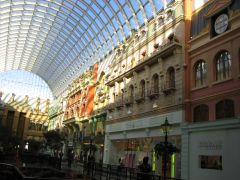
\includegraphics[width=.45\linewidth]{gfx/example_1}} \quad
    \subfloat[Pan ma signo.]
    {\label{fig:example-b}%
        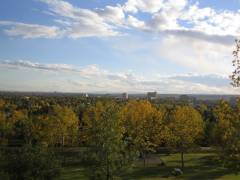
\includegraphics[width=.45\linewidth]{gfx/example_2}} \\
    \subfloat[Methodicamente o uno.]
    {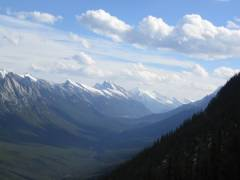
\includegraphics[width=.45\linewidth]{gfx/example_3}} \quad
    \subfloat[Titulo debitas.]
    {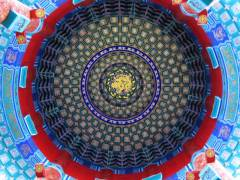
\includegraphics[width=.45\linewidth]{gfx/example_4}}
    \caption[Tu duo titulo debitas latente]{Tu duo titulo debitas
    latente. \ac{DRY}}\label{fig:example}
\end{figure}


%*****************************************
%*****************************************
%*****************************************
%*****************************************
%*****************************************

\chapter{Espressioni regolari}
Le espressioni regolari sono un formalismo comunamente utilizzato per
definire linguaggi semplici.

\begin{theorem}
  La definizione induttiva di un espressione regolare su un alfabeto $A$:
  \paragraph{Base:}
  \begin{itemize}
    \item $0$ è un espressione regolare di $A$;
    \item $\lambda$ è un espressione regolare di $A$;
    \item per ogni $\sigma\in A$, $\sigma$ è un espressione regolare
      in $A$.
  \end{itemize}
  
  \paragraph{Passo induttivo:}
  \begin{itemize}
    \item se $e_1$ ed $e_2$ sono espressioni regolare di $A$,

      allora $e_1|e_2$ è un espressione regolare di $A$;
    \item se $e_1$ ed $e_2$ sono espressioni regolare di $A$,

      allora $e_1 e_2$ è un espressione regolare di $A$;
    \item se $e$ è un espressione regolare di $A$,

      allora $e^\star$ è un espressione regolarare di $A$.
  \end{itemize}
\end{theorem}

\chapter{Analisi sintattica}
\begin{theorem}
  L' \textbf{analisi sintattica} è definita sull'analisi lessicale, risolve:
  \begin{itemize}
    \item il riconoscimento di una sequenza di \emph{lexems/tokens} come
      validi se rispettano alcune regole sintattiche;
    \item la costruzione, in caso di successo, di una rappresentazione
      astratta della sequenza riconosciuta per eseguire delle operazioni su
      di essa.
  \end{itemize}
\end{theorem}

\section{Parser}
\begin{theorem}
  Un \textbf{parser} è un programma che esegue l'analisi sintattica.
\end{theorem}

\subsection{Parsers per i linguaggi di programmazione}
I parser per i linguaggi di programmazione, riconoscono i \emph{token}
generati da un \emph{tokenizer}, mentre le regole sintattiche sono definite
formalmente da una \emph{grammatica}.

I parser generano:
\begin{itemize}
  \item un albero \textbf{parse/deviation}, una rappresentazione meno astratta
    della sequenza analizzata;
  \item un \textbf{albero sintattico astratto} (abstract syntax tree, AST),
    una rappresentazione pi
     astratta della sequenza analizzata.
\end{itemize}

Inoltre i parser possono essere scritti a mano, oppure generati automaticamente
da una grammatica con specifici software come \emph{ANTLR} o \emph{BISON}.

\paragraph{Primo esempio con sintassi C/Java/C++}
Token analizzati:
\begin{itemize}
  \item \emph{IDENTIFIER}: con il nome $"x2"$;
  \item \emph{ASSIGN\_OP};
  \item \emph{INT\_NUMBER}: con il valore di $34$;
  \item \emph{STATEMENT\_TERMINATOR}.
\end{itemize}

Il parser ritornerà errore dato che la sequenza non è riconosciuta oppure
uno o più messaggi di errore sono presenti.


\paragraph{Secondo esempio con sintassi C/Java/C++}
Token analizzati:
\begin{itemize}
  \item \emph{IDENTIFIER}: con il nome $"x2"$;
  \item \emph{ASSIGN\_OP};
  \item \emph{INT\_NUMBER}: con il valore di $34$;
  \item \emph{ADD\_OP};
  \item \emph{INT\_NUMBER}: con il valore di $10$;
  \item \emph{STATEMENT\_TERMINATOR}.
\end{itemize}

Il parser riconosce la sequenza e genera un \emph{AST}.

\begin{figure}[ht]
    \centering
    \incfig{ast}
    \caption{L'AST generato della sequenza precedente.}
    \label{fig:ast-2}
\end{figure}

\chapter{Context free (CF) grammars}
Le grammatiche \emph{context free}, sono il formalismo più diffuso per definire
le regole sintattiche di un linguaggio di programmazione.
Sono più espressive di un espressione regolare e sono basate sulla
concatenazione d unzione di più nomi e su definizioni ricorsive.

\paragraph{Un primo esempio:}
\begin{lstlisting}[language=Java, caption={Una grammatica \textbf{CF} per espressioni semplici}]
Exp ::= Num | Exp '+' Exp | Exp '*' Exp | '(' Exp ')'
Num ::= '0' | '1'
\end{lstlisting}

\paragraph{Da notare che:}
\emph{Num} è definito nella grammatica solo per completezza, infatti i token
\emph{Num} sono definiti separatamente da un espressione regolare.

\begin{lstlisting}[language=Java, caption={Esempio rivisitato di una grammatica
\textbf{CF} per espressioni semplici}]
Exp ::= Num | Exp '+' Exp | Exp '*' Exp | '(' Exp ')'
NUM definito da 0|1
\end{lstlisting}

\paragraph{Notazione:}
In \emph{Exp} è maiuscolo solo il primo carattere: è definito nella grammatica.
In \emph{NUM} tutte le lettere sono maiuscole; è definito separatamente da un
espressione regolare.

\section{Terminologia delle grammatiche CF}
\begin{lstlisting}[language=Java, caption={Esempio}]
Exp ::= Num | Exp '+' Exp | Exp '*' Exp | '(' Exp ')'
Num ::= '0' | '1'
\end{lstlisting}

\subsection{Terminologia per la grammatica G}
Per $G=(T,N,P)$:
\begin{itemize}
  \item $\{'+','*','(',')','0','1'\}$ è l'insieme $T$ dei \textbf{simboli
    terminali};
  \item $\{Exp,Num\}$ sono l'insieme $N$ di simboli \textbf{non terminali};
  \item $\{(Exp,Num),(Exp,Exp,'+'Exp),(Exp,Exp '*'Exp),(Exp,'('Exp')'),(Num,'0'
    ),(Num,'1')\}$ è l'insieme $P$ di produzioni.
\end{itemize}
\paragraph{Da notare che:}
\begin{itemize}
  \item ogni simbolo non terminale corrisponde ad un linguaggio; i linguaggi
    sono definiti come unioni di concatenazioni;
  \item i simboli terminali sono \emph{lexems} dei linguaggi definiti dalla
    grammatica;
  \item le produzioni hanno forma $(B,\alpha)$, per $B\in\N\cap\alpha\in
    (T\cup N)^*$
\end{itemize}

\section{Grammatiche come definizione induttiva di linguaggi}
\subsection{Primo esempio}
\begin{lstlisting}[language=Java, caption={Esempio}]
Exp ::= Num | Exp '+' Exp | Exp '*' Exp | '(' Exp ')'
Num ::= '0' | '1'
\end{lstlisting}

\subsubsection{Definizione induttiva di linguaggi}
\[
  Exp=Num\cup(Exp\cdot\{"+"\}\cdot Exp)\cup(Exp\cdot\{"*"\}\cdot Exp)\cup(\{"("
  \}\cdot Exp\cdot\{")"\})
\]
\[
  Num=\{"0"\}\cup\{"1"\}
\]

\paragraph{Da notare che:}
\begin{itemize}
  \item $Exp=Num\cup\dots$ è il caso base per $Exp$: un numero è un
    espressione;
  \item $Exp$ è definito su di $Num$, $Num$ è definito esclusivamente per casi
    base.
\end{itemize}

\subsection{Secondo esempio}
\begin{lstlisting}[language=Java, caption={Esempio}]
Exp ::= Term | Exp '+' Term | Exp '*' Term
Term ::= '(' Exp ')' | Num
Num ::= '0' | '1'
\end{lstlisting}

\paragraph{Da notare che:}
Le definizioni di $Exp$ e $Term$ sono ricorsive reciprocamente.

\section{Derivazioni}
\begin{lstlisting}[language=Java, caption={Esempio}]
Exp ::= Num | Exp '+' Exp | Exp '*' Exp | '(' Exp ')'
Num ::= '0' | '1'
\end{lstlisting}

\subsection{Linguaggi generati da una grammatica}
\begin{itemize}
  \item Una grammatica genera un linguaggio per ogni simbolo non terminale;
  \item la grammatica precedente genera due linguaggi $L_{\text{Exp}}$ e
    $L_{\text{Num}}$;
  \item il linguaggio per $Num$ è relativamente semplice: $L_{\text{Num}}=
    \{"0","1"\}$.
\end{itemize}

\paragraph{Da notare che:}
per definire $L_{\text{Num}}$ e per dimostrare che $"1+0"\in L_{\text{Exp}}$ e
che $"1+*("\not\in L_{\text{Exp}}$ si rendono necessarie la \textbf{derivazione
a passo singolo e la derivazione a passi multipli}.

\subsection{Derivazione ad un passo}
\begin{itemize}
  \item $Exp\rightarrow Exp'*'Exp$ è usata la produzione $(Exp,Exp '*'Exp)$;
  \item $Exp'*'Exp\rightarrow Num'*'Exp$ è usata la produzione $(Exp,Num)$;
  \item $Num'*'Exp\rightarrow Num'*'Num$ è usata la produzione $(Exp,Num)$;
  \item $Num'*'Num\rightarrow '0''*'Num$ è usata la produzione $(Num,'0')$;
  \item $'0''*'Num\rightarrow '0''*''1'$ è usata la produzione $(Num,'1')$;
\end{itemize}

\paragraph{Da notare che:}
Non esiste alcuna derivazione da $'0''*''1'$ dato che nessuna produzione può
essere usata; $'0''*''1'$ è la stringa $0*1$ che appartiene a $L_{\text{Exp}}$.

\subsection{Definizioni di derivazione}
\subsubsection{Derivazione ad un passo}
\begin{theorem}
  La derivazione ad un passo per la grammatica $G=(T,N,P)$:
  \begin{itemize}
    \item possiede una forma $\alpha_1 B\alpha_2\rightarrow\alpha_1\gamma
      \alpha_2$;
    \item $\alpha_1,\alpha_2\in(T\cup N)^*$;
    \item $(B,\gamma)\in P$ ovvero $(B,\gamma)$ in produzione.
  \end{itemize}
\end{theorem}

\subsubsection{Derivazione a più passi}
\begin{theorem}
  La chiusura transitiva di $\rightarrow$:
  \begin{itemize}
    \item il caso base: se $\gamma_1\rightarrow\gamma_2$, allora $\gamma_1
      \rightarrow^+\gamma_2$;
    \item caso induttivo: se $\gamma_1\rightarrow\gamma_2$, e $\gamma_2
      \rightarrow^+\gamma_3$, allora $\gamma_1\rightarrow^+\gamma_3$.
  \end{itemize}
\end{theorem}

\subsubsection{Linguaggio generato}
Il linguaggio $L_B$ generato da $G=(T,N,P)$ per i non terminali $B\in N$:
\begin{itemize}
  \item tutte le stringhe di terminali che possono essere derivati in uno
    o più passaggi da $B$;
  \item formalmente: $L_B=\{u\mid B\rightarrow^+ u\}$.
\end{itemize}

\subsection{Albero di derivazione (parse tree)}
\paragraph{Osservazione 1}
Le grammatiche CF sono utilizzate per definire linguaggi ed implementare
parsers, i parsers dovrebbero generare gli alberi, ma le derivazioni non
sono alberi.

\paragraph{Osservazione 2}
Un passo di derivazione è determinato da:
\begin{itemize}
  \item la produzione usata;
  \item lo specifico simbolo non termitale che rimpiazza.
\end{itemize}
Quest'ultimo punto non influenza la stringa finale dei terminali ottenuti
dalla derivazione.

\paragraph{Intuizione}
Un albero di derivazione è una generalizzazione di una derivazione a più
passaggi in modo che la stringa derivata contenga solo terminali e che i non
terminali siano rimpiazzati in parallelo.

\subsection{Esempi di alberi di derivazione (ANTLR)}
\begin{lstlisting}[language=Java, caption={Grammatica ANTLR}]
grammar SimpleExp;

Exp ::= Num | Exp '+' Exp | Exp '*' Exp | '(' Exp ')'
Num ::= '0' | '1'
\end{lstlisting}

\subsubsection{Albero di derivazione per "1*1+1"}
\begin{figure}[ht]
    \centering
    \incfig{dtree-1}
    \caption{Albero di derivazione per "1*1+1""}
    \label{fig:dtree-1}
\end{figure}

\chapter{Alberi di derivazione}
\section{Albero di derivazione (parse tree)}
\paragraph{Osservazione 1}
Le grammatiche CF sono utilizzate per definire linguaggi ed implementare
parsers, i parsers dovrebbero generare gli alberi, ma le derivazioni non
sono alberi.

\paragraph{Osservazione 2}
Un passo di derivazione è determinato da:
\begin{itemize}
  \item la produzione usata;
  \item lo specifico simbolo non termitale che rimpiazza.
\end{itemize}
Quest'ultimo punto non influenza la stringa finale dei terminali ottenuti
dalla derivazione.

\paragraph{Intuizione}
Un albero di derivazione è una generalizzazione di una derivazione a più
passaggi in modo che la stringa derivata contenga solo terminali e che i non
terminali siano rimpiazzati in parallelo.

\subsection{Esempi di alberi di derivazione (ANTLR)}
\begin{lstlisting}[language=Java, caption={Grammatica ANTLR}]
grammar SimpleExp;

Exp ::= Num | Exp '+' Exp | Exp '*' Exp | '(' Exp ')'
Num ::= '0' | '1'
\end{lstlisting}

\subsubsection{Albero di derivazione per "1*1+1"}
\begin{figure}[h]
    \centering
    \incfig{dtree-1}
    \caption{Albero di derivazione per "1*1+1""}
    \label{fig:dtree-1}
\end{figure}

\paragraph{Esercizio:}
Mostrare che $"1*1+1"\in L_{\text{Exp}}$ usando la nozione di
derivazione ad uno o più passi.
\[
  Exp\rightarrow Exp'+'Exp\rightarrow^+ Exp\times Exp'+'Num'
  \rightarrow^+ Num'*'Num'+'1'
  \rightarrow^+ \text{'1' '*' '1' '+' '1'}
\]
\paragraph{Esercizio:}
Mostrare che $"1+(\not\in L_{\text{Exp}}$:
\[
  Exp\rightarrow Exp '*' Exp\rightarrow^+ Num '*' Exp '+' Exp \rightarrow^+
\text{'1' '*' Num '+' Num}\rightarrow^+\text{'1' '*' '1' '+' '1'}
\]

\subsection{Definizione di albero di derivazione in G=(T,N,P)}
Albero di derivazione per $u\in T^*$ partendo da $B\in N$.
\begin{itemize}
  \item se un nodo è etichettato da $C$ ed ha $n$ figli $I_1,\dots,I_n$,
    allora $(C,I_1,\dots,I_n)\in P$ (ovvero, $(C,I_1,\dots,I_n)$ è una
    produzione di $G$;
  \item la radice è etichettata da $B$;
  \item $u$ è ottenuto dalla concatenaziona da sinistra a destra dii tutte le
    etichette terminali (nodi foglia).
\end{itemize}

\subsubsection{Definizione equivalente di un linguaggio generato}
Il linguaggio $L_B$ generato da $G=(T,N,P)$ per un non terminale $B\in N$ è
composto da tutte le stringhe $u$ di terminali così che esiste un albero di
derivazione per $u$ partendo da $B$.

\chapter{Grammatiche ambigue}
\begin{theorem}
  Una grammatica $G=(T,N,P)$ è ambigua per $B\in N$ se esitono due differenti
  alberi di derivazione partendo da $B$ per la stessa stringa.
\end{theorem}

Per esempio la grammatica $1+1+1$ è ambigua a seconda delle parentesi.

\section{Soluzioni per l'ambiguità}
Per risolvere il problema dell'ambiguità si può cambiare la sintassi:
\subsection{Notazione prefissa}
\begin{lstlisting}[language=Java, caption={Notazione prefissa}]
Exp ::= Num | '+' Exp Exp | '*' Exp Exp
Num ::= '0' | '1'
\end{lstlisting}

In questo caso esiste un unico albero di derivazione per $"1 1+1*$ e le
parentesi non sono più necessarie.

\subsection{Notazione postfissa}
\begin{lstlisting}[language=Java, caption={Notazione postfissa}]
Exp ::= Num | Exp Exp '+' | Exp Exp '*'
Num ::= '0' | '1'
\end{lstlisting}

In questo caso esiste di nuovo un unico albero di derivazione e le parentesi
sono di nuovo non necessarie.
 
\subsection{Notazione funzionale}
\begin{lstlisting}[language=Java, caption={Notazione funzionale}]
Exp ::= Num | 'add' '(' Exp ',' Exp ')' | 'mul' '(' Exp ',' Exp ')'
Num ::= '0' | '1'
\end{lstlisting}

In questo esempio esiste un unico albero di derivazione per $add(1,mul(1,1)$.

\subsection{Notazione infissa}
Generalmente la notazione infissa è una soluzione più pratica.

\begin{itemize}
  \item si definiscono le regole di associatività per gli operatori binari:
    \begin{itemize}
      \item addizione associativa a sinistra: $"1+1+1"$ diventa $"(1+1)+1"$;
      \item addizione associativa a destra: $"1+1+1"$ diventa $"1+(1+1)"$;
    \end{itemize}
  \item si definiscono le regole di precedenza per gli operatori, usando
    le parentesi per sovrascriverlo:
    \begin{itemize}
      \item la moltiplicazione ha precedenza rispetto l'addizione: $"1+1*1"$
        significa $"1+(1*1)"$;
      \item l'addizione ha precedenza rispetto la moltiplicazione: $"1*1+1"$
        significa $"1*(1+1)"$.
    \end{itemize}
\end{itemize}

\subsection{Operatori con la stessa precedenza}
Gli operatori binari possono avere la stessa precedenza, in questo caso
condividono la regola associativa:
\begin{itemize}
  \item addizione e moltiplicazione hanno la stessa precedenza e sono
    associative a sinistra: $"1+1*1"$ diventa $"1+(1*1)"$ e $"1*1+1"$ diventa
    $"(1*1)+1"$;
  \item addizione e moltiplicazione hanno la stessa precedenza e sono
    associative a destra: $"1+1*1"$ diventa $"1+(1*1)"$ e $"1*1+1"$ diventa
    $"1*(1+1)"$;
\end{itemize}

\paragraph{Nota che:}
le regole sull' associatività risolvono ambiguità tra operatori binari con la
stessa precedenza, inoltre mischiando operatori con diverse \textbf{arità}
rende l'eliminazione dell'ambiguità più complessa.

\subsection{Tecniche per risolvere l'ambiguità}
\begin{itemize}
  \item una grammatica ambigua $G$ è trasformata in una grammatica non ambigua
    $G^\prime$;
  \item l' \textbf{equivalenza} significa che per tutti i non terminali di
    $B$ e $G$, i linguaggi generati da $G,G^\prime,B$ sono uguali;
  \item è possibile per la \textbf{trasformazione} di codificare l'
    associatività e le regole di precedenza nella grammatica non ambigua
    $G^\prime$.
\end{itemize}

\subsubsection{Esempio 1: + e * con la stessa precedenza}
\begin{lstlisting}[language=Java, caption={Grammatica ambigua}]
Exp ::= Num | Exp '+' Exp | Exp '*' Exp | '(' Exp ')'
Num ::= '0' | '1'
\end{lstlisting}

\begin{lstlisting}[language=Java, caption={Associatività a sinistra non ambigua}]
Exp ::= Atom | Exp '+' Atom | Exp '*' Atom
Atom ::= Num | '(' Exp ')'
Num ::= '0' | '1'
\end{lstlisting}
Nota che: $Exp '+' Atom | Exp '*' Atom$ significa che sul lato destro di
$+(*)$, le addizione (e moltiplicazioni) sono permesse solo se circondate da
parentesi.

\begin{tikzpicture}[sibling distance=10em,
  every node/.style = {shape=rectangle, rounded corners, draw, align=center}]]
  \node {exp}
    child { node {exp} 
      child { node {exp}
        child { node {atom}
          child { node {num} 
            child { node {1} }
          }
        }
      }
      child { node {+} }
      child { node {atom}
        child { node {num}
          child {node {1} }
        }
      }
    }
    child { node{*} }
    child { node{atom}
      child { node {num}
        child { node {1} }
      }
    };
\end{tikzpicture}

\begin{lstlisting}[language=Java, caption={Associatività a destra non ambigua}]
Exp ::= Atom | Atom '+' Exp | Atom '*' Exp
Atom ::= Num | '(' Exp ')'
Num ::= '0' | '1'
\end{lstlisting}
Nota che: $Atom '+' Exp | Atom '*' Exp$ significa che sul lato sinistro di 
$+(*)$,le addizione (e moltiplicazioni) sono permesse solo se circondate da
parentesi.
\begin{figure}[H]
  \centering
  \resizebox{.5\textwidth}{!}{%
\begin{tikzpicture}[sibling distance=4em,
  every node/.style = {shape=rectangle, rounded corners, draw, align=center}]
  \node {exp}
    child { node{atom}
      child { node {num}
        child { node {1} }
      }
    }
    child { node{+} }
    child { node {exp} 
      child { node {atom}
        child { node {num}
          child {node {1} }
        }
      }
      child { node {*} }
      child { node {exp}
        child { node {atom}
          child { node {num} 
            child { node {1} }
          }
        }
      }
    };
\end{tikzpicture}
}
\end{figure}

\subsubsection{Esempio 2: * con la maggiore precedenza}
\begin{lstlisting}[language=Java, caption={Associative a sinistra non ambigue}]
Exp ::= Mul | Exp '+' Mul
Mul ::= Atom | Mul '*' Atom'
Atom ::=  Num | '(' Exp ')'
Num ::= '0' | '1'
\end{lstlisting}
Nota che: $Mul '*' Atom $ significa che entrambi i lati delle addizione di $*$
sono permesse solo se circondate da parentesi.

\begin{lstlisting}[language=Java, caption={Associative a destra non ambigue}]
Exp ::= Mul | Exp '+' Mul
Mul ::= Atom | Atom '*' Mul'
Atom ::=  Num | '(' Exp ')'
Num ::= '0' | '1'
\end{lstlisting}
Nota che: $Atom '*' Mul $ significa che entrambi i lati delle addizione di $*$
sono permesse solo se circondate da parentesi.

\subsubsection{Esempi rimanenti}
\begin{itemize}
  \item $*$ con precedenza ed associativtà  a sinistra, $+$ associatività a
    destra;
  \item $*$ con precedenza ed associativtà  a destra, $+$ associatività a
    sinistra;
  \item $+$ con precedenza ed associativtà  a sinistra, $*$ associatività a
    destra;
  \item $+$ con precedenza ed associativtà  a destra, $+$ associatività a
    sinsitra;
\end{itemize}

\section{Sintassi ambigua per statements}
\begin{lstlisting}[language=Java, caption={Esempio di ambiguità per gli statements}]
Stmt ::= ID '=' Exp | 'if' '(' Exp ')' Stmt | Stmt ';' Stmt | '{' Stmt '}'
Exp ::= ID | BOOL // ID e BOOL sono definiti da espressioni regolari
\end{lstlisting}

\begin{figure}[H]
  \caption{Primo esempio di albero di derivazione per "if(x) x=false;y=true"}
  \centering\resizebox{\textwidth}{!}{%
\begin{tikzpicture}[
  level 1/.style = {sibling distance=8em},   % <-- added
  level 2/.style = {sibling distance=4em},    % <-- added
  level 3/.style = {sibling distance=2em},    % <-- added
  every node/.style = {
    shape=rectangle,
    rounded corners,
    draw,
    align=center
  }]
  \node {stmt}
    child { node {stmt}
      child { node {if} }
      child { node {$($} }
      child { node {exp}
        child { node {x} }
      }
      child { node {$)$} }
      child { node {stmt}
        child { node {x}}
        child { node {=} }
        child { node {exp}
          child { node {false} }
        }
      }
    }
    child { node {;} }
    child { node {stmt}
      child { node {y} }
      child { node {=} }
      child { node {exp}
        child { node {true} }
      }
    };
\end{tikzpicture}}\end{figure}
\begin{figure}[H]
  \caption{Secondo esempio di albero di derivazione per "if(x) x=false;y=true"}
  \centering\resizebox{\textwidth}{!}{%
\begin{tikzpicture}[
  level 1/.style = {sibling distance=4em},   % <-- added
  level 2/.style = {sibling distance=4em},    % <-- added
  level 3/.style = {sibling distance=2em},    % <-- added
  every node/.style = {
    shape=rectangle,
    rounded corners,
    draw,
    align=center
  }]
  \node {stmt}
    child { node {if} }
    child { node {$($} }
    child { node {exp}
      child { node {x} }
    }
    child { node {$)$} }
    child { node {stmt}
      child { node {stmt}
        child { node {x} }
        child { node {=} }
        child { node {exp}
          child { node {false} }
        }
      }
    }
    child { node {;} }
    child { node {stmt}
      child { node {y} }
      child { node {=} }
      child { node {exp}
        child { node {true} }
      }
    };
\end{tikzpicture}}\end{figure}



\chapter{Costruzione di un parser da una grammatica}
Individuiamo due passaggi per costruire un parser da una grammatica:
\begin{enumerate}
  \item la grammatica non deve essere ambigua;
    \begin{lstlisting}[language=Java, caption={Una grammatica non ambigua}]
    Exp ::= Mul | Exp '+' Mul
    Mul ::= Atom | Mul '*' Atom
    Atom ::= Num | '(' Exp ')'
    Num ::= '0' | '1'
    \end{lstlisting}
  \item per ogni token di input, il parser dever sceltiere una
    produzione unica da usare per l'albero \emph{parse} corretto.
\end{enumerate}

\paragraph{Problemi:}
\begin{itemize}
  \item i token sono letti dal parser da sinsitra a destra;
  \item nella più semplice delle ipotesi, il parser è a conoscenza
    solo del token successivo (\emph{lookahead token});
  \item un parser con un \emph{lookahead token} non è in grado di
    scegliere la giusta produzione per la grammatica di cui sopra.
\end{itemize}

\section{Come costruire un parser da una grammatica}
\begin{lstlisting}[language=Java, caption={Una grammatica non ambigua}]
  Exp ::= Mul | Exp '+' Mul
  Mul ::= Atom | Mul '*' Atom
  Atom ::= Num | '(' Exp ')'
  Num ::= '0' | '1'
\end{lstlisting}
Quindi un parser con \textbf{un} \emph{lookahead token} non può essere
costruito per la grammatica di cui sopra.
\paragraph{Controesempio:}
Se il primo lookahead token è un numero, allora entrambe le produzioni di
\emph{Exp} potrebbero funzionare.
A seconda del secondo lookahead token $t$:
\begin{itemize}
  \item la produzione ($Exp$,$Mul$) è usata se $t$ è $'*'$ oppure la fine
    dello stream di input;
  \item la produzione ($Exp$,$Exp$ $'+'$ $Mul$) è usata se $t='+'$.
\end{itemize}

\subparagraph{Osservazioni:}
Per costruire un albero \emph{parse}, la produzione ($Exp$,$Mul$) deve essere
usata, inoltre quando le produzioni di $Exp$ sono usate consecutivamente,
vengono ottenute stringhe della forma seguente: $Mul$, oppure $Mul$ seguita
dalla stringa $'+'Mul$ ripetuta una o più volte.

\begin{lstlisting}[language=Java, caption={Grammatica rivisitata a seguito delle osservazioni precedenti}]
  Exp ::= Mul | AddSeq
  AddSeq ::= '+' Mul | '+' Mul AddSeq
  Mul ::= Atom | Mul '*' Atom
  Atom ::= Num | '(' Exp ')'
  Num ::= '0' | '1'
\end{lstlisting}

\paragraph{Considerazioni sulla trasformazione della grammatica}
La grammatica è equivalente alla precedente, ma quando si costruisce un albero
\emph{parse} sappiamo che un nodo $Exp$ deve sempre avere un figlio $c$ a
sinistra etichettato da $Mul$ dopo che l'albero \emph{parse} con radice $c$ è
stato costruito, quindi la produzione corretta è ($Exp$, $Mul$ $AddSeq$) se
il token \emph{lookahead} è $'+'$;
altrimenti la produzione è ($Exp$,$Mul$): un nodo $AddSeq$ deve sempre avere un
figlio a sinistra $c_1$ etichettato da $'+'$, seguito da un figlio $c_2$
etichettato da $Mul$.

Dopo che l'albero con radice $c_2$  è costruito, la produzione corretta se
il token \emph{lookahead}$='+'$ è: ($AddSeq$, $'+'$ $Mul$ $AddSeq$), altrimenti
la produzione è ($AddSeq$, $'+'$ $Mul$).

\begin{lstlisting}[language=Java, caption={Soluzione completa}]
  Exp ::= Mul | AddSeq
  AddSeq ::= '+' Mul | '+' Mul AddSeq
  Mul ::= Atom | Atom MulSeq
  MulSeq ::= '*' Atom | '*' Atom MulSeq
  Atom ::= Num | '(' Exp ')'
  Num ::= '0' | '1'
\end{lstlisting}

\begin{figure}[H]
\caption{Parse tree per "1+1*1"}
\centering\resizebox{.5\textwidth}{!}{%
\begin{tikzpicture}[%
  level 1/.style = {sibling distance=8em},   % <-- added
  level 2/.style = {sibling distance=4em},    % <-- added
  level 3/.style = {sibling distance=5em},    % <-- added
  every node/.style = {
    shape=rectangle,
    rounded corners,
    draw,
    align=center
  }]
  \node {exp}
    child { node {mul}
      child { node {atom}
        child { node {num}
          child { node {1} }
        }
      }
    }
    child { node {AddSeq}
      child { node {+} }
      child { node {mul}
        child { node {atom}
          child { node {num}
            child { node {1} }
          }
        }
        child { node {MulSeq}
          child { node {*} }
          child { node {atom}
            child { node {num}
              child { node {1} }
            }
          }
        }
      }
    };
\end{tikzpicture}}\end{figure}

\chapter{Paradigmi di programmazione}
\begin{theorem}
  I paradigmi di programmazione sono lo stile/approccio nell'utilizzo di un
  linguaggio di programmazione.
\end{theorem}

Il più delle volte un paradigma di programmazione è basato un un modello
computazionale emergente.

\paragraph{Esempi principali di paradigmi}
\begin{itemize}
  \item \textbf{Imperativi:} più vicini al modello hardware, quindi basati
    sulle nozioni di istruzione e stato, dei linguaggi di esempio sono:
    \begin{itemize}
      \item \textit{proceduali:} C;
      \item \textit{orientati agli oggetti:} Java;
    \end{itemize}
  \item \textbf{dichiarativi:} basati su un modello astratto, esempi di
    linguaggi sono:
    \begin{itemize}
      \item \textit{funzionali:} \emph{ML}, basati sulla nozione di
        \emph{definizione di funzione} e \emph{applicazione di funzione};
      \item \textit{logici:} \emph{Prolog}, basati sulla nozione di \emph{
        regola logica} e \emph{query}.
    \end{itemize}
\end{itemize}

Di solito i linguaggi di programmazione implementano più di un paradigma per
favorire la flessibilità, \emph{Java, Javascript, Python} supportano sia
i paradigmi imperativi che quelli dichiarativi.

\section{Paradigma completamente funzionale}
Caratteristiche:
\begin{itemize}
  \item \textbf{programma:} le definizioni di funzioni matematiche ed un
    espressione principale;
  \item \textbf{computazione:} l'applicazione della funzione (\emph{function
    call});
  \item \textbf{nessuna nozione di stato:} nessun assegnamento di variabili,
    più in generale nessuno \emph{statement}, solo \emph{espressioni};
  \item \textbf{variabili:} parametri di funzioni o variabili locali
    contenenti valori costanti.
\end{itemize}

Terminologia:
\begin{itemize}
  \item \textbf{higher order functions:} funzioni che possono accettare
    funzioni come argomenti e possono ritornare funzioni;
  \item \textbf{lambda expression/fuunction o anonymous functions:} funzioni
    ottenuto dall'evaluazione di un espressione.
\end{itemize}

\paragraph{Le funzioni sono valori di prima classe:}
un evaluazione di espressioni può dare come risultato un altra espressione 
(first class values).

\section{OCaml}
OCaml deriva da \textbf{ML}, è un linguaggio multi-paradigma con un approccio
puramente funzionale, è staticamente tipato con inferenza di tipo:
\begin{itemize}
  \item gli errori di tipo sono rilevati staticamente;
  \item i tipi possono essere omessi nei programmi.
\end{itemize}

\begin{lstlisting}[language=Caml, caption={Sintassi}]
Exp ::= ID | NUM | Exp Exp | 'fun' Pat+ '->' Exp | UOP Exp | Exp BOP Exp | '(' Exp ')'
Pat ::= ID // pattern semplificato
\end{lstlisting}

\paragraph{Commenti:}
\begin{itemize}
  \item \textbf{ID} rappresenta gli identificatori di variabile $[a-zA-Z\_]
    [\backslash w']*$;
  \item \textbf{NUM} rappresenta i numeri naturali:
    \[
      0[bB][01][01\_]*|0[oO][0-7][0-7\_]*|0[xX][0-9a-fA-F][0-9a-fA-F\_]*|\backslash d[\backslash d\_]*
    \];
  \item \textbf{UOP} rappresenta operatori aritmetici unari $[+-]$;
  \item \textbf{BOP} rappresenta operatori aritmetici binari $[+-*\backslash]|mod$;
  \item \textbf{Pat} rappresenta i patterns, per semplicità si possono
    associare agli identificatori.
\end{itemize}

\subsection{Funzioni ed applicazioni}
\begin{itemize}
  \item esempi di funzioni anonime:
    \begin{lstlisting}[language=Caml, caption={Esempio di funzioni anonime}]
    fun x -> x+1 (* funzione di incremento *)
    fun x y -> x+y (* funzione di addizione *)
    \end{lstlisting}
  \item applicazione di funzioni:
    \begin{lstlisting}[language=Caml, caption={Esempio di applicazione di funzioni}]
    (fun x -> x+1) 3 (* il risultato sara 4 *)
    \end{lstlisting}
\end{itemize}

Inoltre prendendo in esempio:
\begin{lstlisting}[language=Caml, caption={Esempio di applicazioni}]
  exp1 exp2
\end{lstlisting}
\begin{itemize}
  \item l'evaluazione di \textbf{exp1} si aspetta come valore di ritorno una
    funzione $f$;
  \item l'evaluazione di \textbf{exp2} si aspetta come valore di ritorno un
    argomento valido $a$;
  \item l'evaluazione di \textbf{exp1 exp2} ritorna $f(a)$ ($f$ applicato ad
    $a$).
\end{itemize}

\subsection{Regole di precedenza ed associatività}
\begin{itemize}
  \item Si usano le regole standard per le espressioni aritmetiche;
  \item l'applicazione è associativa a sinistra:
    \begin{lstlisting}[language=Caml, caption={Esempio di associatività}]
    (fun x y -> x+y) 3 4 (* equivale a ((fun x y -> x+y) 3) 4 *)
    \end{lstlisting}
  \item l'applicazione ha precedenza maggiore rispetto gli operatori binari:
    \begin{lstlisting}[language=Caml, caption={Esempio di precedenza}]
    (fun x -> x*2) 1+2 (* equivale a ((fun x -> x*2) 1) +2 *)
    1+(fun x -> x*2) 1+2 (* equivale a 1+((fun x -> x*2) 1) +2 *)
    \end{lstlisting}
  \item le funzioni anonime hanno piorità più bassa rispetto le applicazioni
    e gli operatori binari:
    \begin{lstlisting}[language=Caml, caption={Esempio di precedenza}]
    fun x -> x*2 (* equivale a fun x -> x*2) *)
    fun f a -> f a (* equivale a fun f a -> (f a) *)
    \end{lstlisting}
  \item i casi limite:
    \begin{lstlisting}[language=Caml, caption={Casi limite di precedenza}]
    f + 3 (* addizione *)
    f (+3) (* applicazione *)
    f - 3 (* sottrazione *)
    f (-3) (* applicazione *)
    + f 3 (* equivale a +(f 3) *)
    - f 3 (* equivale a -(f 3) *)
    \end{lstlisting}

\end{itemize}

\part{Ocaml}\label{pt:ocaml}
\chapter{OCaml}
OCaml deriva da \textbf{ML}, è un linguaggio multi-paradigma con un approccio
puramente funzionale, è staticamente tipato con inferenza di tipo:
\begin{itemize}
  \item gli errori di tipo sono rilevati staticamente;
  \item i tipi possono essere omessi nei programmi.
\end{itemize}

\begin{lstlisting}[language=Caml, caption={Sintassi}]
Exp ::= ID | NUM | Exp Exp | 'fun' Pat+ '->' Exp | UOP Exp | Exp BOP Exp | '(' Exp ')'
Pat ::= ID // pattern semplificato
\end{lstlisting}

\paragraph{Commenti:}
\begin{itemize}
  \item \textbf{ID} rappresenta gli identificatori di variabile $[a-zA-Z\_]
    [\backslash w']*$;
  \item \textbf{NUM} rappresenta i numeri naturali:
    \[
      0[bB][01][01\_]*|0[oO][0-7][0-7\_]*|0[xX][0-9a-fA-F][0-9a-fA-F\_]*|\backslash d[\backslash d\_]*
    \];
  \item \textbf{UOP} rappresenta operatori aritmetici unari $[+-]$;
  \item \textbf{BOP} rappresenta operatori aritmetici binari $[+-*\backslash]|mod$;
  \item \textbf{Pat} rappresenta i patterns, per semplicità si possono
    associare agli identificatori.
\end{itemize}

\section{Funzioni ed applicazioni}
\begin{itemize}
  \item esempi di funzioni anonime:
    \begin{lstlisting}[language=Caml, caption={Esempio di funzioni anonime}]
    fun x -> x+1 (* funzione di incremento *)
    fun x y -> x+y (* funzione di addizione *)
    \end{lstlisting}
  \item applicazione di funzioni:
    \begin{lstlisting}[language=Caml, caption={Esempio di applicazione di funzioni}]
    (fun x -> x+1) 3 (* il risultato sara 4 *)
    \end{lstlisting}
\end{itemize}

Inoltre prendendo in esempio:
\begin{lstlisting}[language=Caml, caption={Esempio di applicazioni}]
  exp1 exp2
\end{lstlisting}
\begin{itemize}
  \item l'evaluazione di \textbf{exp1} si aspetta come valore di ritorno una
    funzione $f$;
  \item l'evaluazione di \textbf{exp2} si aspetta come valore di ritorno un
    argomento valido $a$;
  \item l'evaluazione di \textbf{exp1 exp2} ritorna $f(a)$ ($f$ applicato ad
    $a$).
\end{itemize}

\section{Regole di precedenza ed associatività}
\begin{itemize}
  \item Si usano le regole standard per le espressioni aritmetiche;
  \item l'applicazione è associativa a sinistra:
    \begin{lstlisting}[language=Caml, caption={Esempio di associatività}]
    (fun x y -> x+y) 3 4 (* equivale a ((fun x y -> x+y) 3) 4 *)
    \end{lstlisting}
  \item l'applicazione ha precedenza maggiore rispetto gli operatori binari:
    \begin{lstlisting}[language=Caml, caption={Esempio di precedenza}]
    (fun x -> x*2) 1+2 (* equivale a ((fun x -> x*2) 1) +2 *)
    1+(fun x -> x*2) 1+2 (* equivale a 1+((fun x -> x*2) 1) +2 *)
    \end{lstlisting}
  \item le funzioni anonime hanno piorità più bassa rispetto le applicazioni
    e gli operatori binari:
    \begin{lstlisting}[language=Caml, caption={Esempio di precedenza}]
    fun x -> x*2 (* equivale a fun x -> x*2) *)
    fun f a -> f a (* equivale a fun f a -> (f a) *)
    \end{lstlisting}
  \item i casi limite:
    \begin{lstlisting}[language=Caml, caption={Casi limite di precedenza}]
    f + 3 (* addizione *)
    f (+3) (* applicazione *)
    f - 3 (* sottrazione *)
    f (-3) (* applicazione *)
    + f 3 (* equivale a +(f 3) *)
    - f 3 (* equivale a -(f 3) *)
    \end{lstlisting}
\end{itemize}

\section{Una sessione REPL (Read Eval Print Loop)}
\begin{lstlisting}[language=Caml, caption={I tipi possono essere inferiti dall'interprete}]
# 42;;
- : int = 42
# fun x->x*2;;
- : int -> int = <fun>
# (fun x->x+1) 2;;
- : int = 3
\end{lstlisting}

\section{Sintassi}
\begin{lstlisting}[language=Caml, caption={Grammatica BNF}]
Type ::= 'int' | Type '->' Type
\end{lstlisting}

\subsection{Terminologia}
\begin{itemize}
  \item \textbf{int} è il tipo primitivo degli interi;
  \item \textbf{int} -> \textbf{int} è un tipo composito;
  \item \textbf{->} è un tipo \textit{costruttore}, usato per costruire tipi
    compositi da tipi più semplici;
  \item i tipi costruiti con il costruttore freccia (->) sono chiamati \emph{
    arrow types} o \emph{tipi di funzione}.
\end{itemize}

\paragraph{Significato del tipo freccia}
$t_1 -> t_2$ identifica il tipo di funzioni da $t_1$ a $t_2$ che:
\begin{itemize}
  \item piò essere applicazo ad un singolo argomento di tipo $t_1$;
  \item ritorna sempre un valore di tipo $t_2$.
\end{itemize}

\subparagraph{Osservazioni:}
\begin{itemize}
  \item il costruttore di tipo freccia è associativo a destra.
    \begin{lstlisting}[language=Caml, caption={Associatività a destra dell'operatore freccia}]
    int->int->int = int->(int->int)
    \end{lstlisting}
  \item un tipo costruttore costruisce sempre un tipo diverso rispetto a quello
    dei propri componenti:
    \[
      t_1 \text{->} t_2 \neq t_1 \qquad t_1 \text{->} t_2 \neq t_2
    \]
  \item due tipi freccia sono uguali se sono costruiti dallo stesso tipo di
    componenti:
    \[
      t_1 \text{->} t_2 = t_3 \text{->} t_4 \text{ se e solo se } t_1 = t_3 \cap t_2 = t_4
    \]
  \item dai punti prima deduciamo:
    \begin{lstlisting}[language=Caml, escapeinside={(*}{*)}]
    int->int->int (*$\neq$*) int->(int->int)
    \end{lstlisting}
\end{itemize}

\subsection{Funzioni di alto ordine}
\[
  \textbf{fun } pat_1 pat_2 \dots pat_n \text{->} exp
\]
è un abbreviazione di:
\[
  \textbf{fun } pat_1 \text{->}\textbf{fun }pat_2 \text{->}\dots \textbf{fun }pat_n \text{->} exp
\]
\section{Tuple}
\begin{lstlisting}[language=Caml, escapeinside={(*}{*)}, caption={Nuove
produzioni per Exp e Pat}]
Exp ::= '(' ')' | Exp ',' Exp
Pat ::= '(' ')' | '(' Pat (',' Pat)* ')'
\end{lstlisting}

\begin{lstlisting}[language=Caml, escapeinside={(*}{*)}, caption={Nuova
produzione per Type}]
Type ::= 'unit' | Type '*' Type
\end{lstlisting}

\subsection{Precedenza ed associatività}
\begin{itemize}
  \item l'operatore \emph{tuple} ha precedenza più bassa rispetto gli altri
    operatori;
  \item l'operatore \emph{tuple} non è associativo nè a destra nè a sinistra;
  \item il costruttore $*$ ha precedenza maggiore del costruttore $->$;
  \item il costruttore $*$ non è associativo nè a destra nè a sinistra.
\end{itemize}

\begin{lstlisting}[language=Caml, escapeinside={(*}{*)}, caption={Esempi
di tuple}]
# ()
- : unit = ()

# 1,2,3
- : int * int * int = (1,2,3)

# (1,2),3
- : (int * int) * int = ((1,2),3)

# 1,(2,3)
- : int * (int * int) = (1,(2,3))

# fun() -> 3
- : unit -> int = <fun>

# fun ((x,y),z)->x*y*z
- : (int * int) * int -> int = <fun>

#fun (x. (y,z))->x*y*z
- : int * (int * int) -> int 0 <fun>
\end{lstlisting}

\section{Funzioni curry}
\begin{theorem}
  Una funzione curry (da \emph{Haskell Curry}), è una funzione di alto
  ordine con un singolo argomento che ritorna una catena di funzioni con
  un singolo argomento.

  Una funzione non curry è una funzione con argomenti multipli.
\end{theorem}

Una funzione curry può essere trasformata in una funzione non curry e
viceversa.

\begin{lstlisting}[language=Caml, escapeinside={(£}{£)}, caption={Esempi
di funzioni curry}]
(* addizione di due interi *)
fun x y -> x+y;; (* versione curry int->int->int *)
fun (x y) -> x+y;; (* versione non curry int->int->int *)
(* moltiplicazione di tre interi *)
fun x y z -> x*y*z;; (* versione curry int->int->int->int *)
fun (x y z) -> x*y*z;; (* versione non curry int->int->int->int *)
\end{lstlisting}

\subsection{Applicazione parziale}
Le funzioni curry permettono l'applicazione parziale, ovvero gli argomenti
possono essere passati uno alla volta.

Le funzioni non curry non permettono un applicazione parziale, tutti gli
argomenti devono essere passai.
\begin{lstlisting}[language=Caml, escapeinside={(£}{£)}, caption={Esempi
di applicazione parziale di funzioni curry}]
let curried_add x y=x+y;;
let uncurried_add(x,y)=x+y;;
(* computa 1+2 con la versione non curry *)
uncarried_add(1,2);;
(* computa 1+2 con l'applicazione parziale *)
let inc=curried_add 1;; (* passa l'argomento 1 e salva il risultato *)
inc 2;; (* passa l'argomento 2 e computa il risultato finale *)
\end{lstlisting}

L'applicazione parziale permette la specializzazione di funzioni: da una
funzione generica è possibile generarne di più specifiche senza
duplicazione di codice, quindi il riutilizzo e la mantenibilità sono
favoriti.

\section{Valori booleani}
Per $BOOL=false|true$.
\begin{lstlisting}[language=Caml, escapeinside={(£}{£)}, caption={Sintassi}]
Exp ::= BOOL | 'not' Exp | Exp '&&' Exp | Exp '||' Exp
Type ::= 'bool'
\end{lstlisting}

\subsection{Regole sintattiche standard}
\begin{itemize}
  \item $\&\&$ e $||$ sono associativi a sinistra;
  \item \textbf{not} ha precedenza maggiore di $\&\&$;
  \item $\&\&$ ha precedenza maggiore di $||$.
\end{itemize}

\subsection{Semantica statica}
\begin{itemize}
  \item \textbf{false} e \textbf{true} sono di tipo \emph{bool};
  \item \textbf{not} $e$ è di tipo \emph{bool} se e solo se $e$ è di tipo
    \emph{bool};
  \item il tipo di \textbf{not} $e$ non è corretto se $e$ non è di tipo
    \emph{bool} oppure se il tipo di $e$ non è corretto;
  \item $e_1\&\&e_2$ e $e_1||e_2$ sono di tipo \emph{bool} se e solo se $e_1$
    ed $e_2$ sono di tipo \emph{bool};
  \item il tipo di \textbf{not} $e_1\&\&e_2$ e $e_1||e_2$ non è corretto se
    $e_1$ o $e_2$ non sono di tipo \emph{bool} oppure se il tipo di $e_1$ o
    $e_2$ non è corretto.
\end{itemize}


Inoltre:
\begin{itemize}
  \item gli operatori $\&\&$ e $||$ sono risolti sinistra a destra;
  \item se $e_1$ ritorna \emph{false} allora $e_1\&\&e_2$ ritorna
    \emph{false}, altrimenti ritorna il valore di $e_2$;
  \item se $e_1$ ritorna \emph{true} allora $e_1||e_2$ ritorna \emph{true},
    altrimenti ritorna il valore di $e_2$.
\end{itemize}

\subsection{Espressioni condizionali}
le operazioni condizionali hanno precedenza minore di tutte le altre
operazioni.

\begin{lstlisting}[
  language=Caml,
  escapeinside={(£}{£)},
  caption={
    Espressioni condizionali
  }]
Exp ::= 'if' Exp 'then Exp 'else' Exp
\end{lstlisting}

\subsection{Variabili globali}
\begin{lstlisting}[
  language=Caml,
  escapeinside={(£}{£)},
  caption={
    Grammatica delle variabili globali
  }
]
Dec ::= 'let' Def (' and' Def)*
    | 'let' 'rec' FunDef (' and' FunDef)*
Def ::= Pat '=' Exp | FunDef
FunDef ::= ID Pat* '=' Exp
\end{lstlisting}

\paragraph{Esempio di variabili globali e funzioni curry}
Consideriamo i seguenti due esempi.
\begin{lstlisting}[
  language=Caml,
  escapeinside={(£}{£)},
  caption={
    Addizione di quadrati
  }
]
let rec sumsquare n = (* sumsquare si usa anche con associativo a destra*)
  if n<=0 then 0 else n*n+sumsquare(n-1);;
\end{lstlisting}

\begin{lstlisting}[
  language=Caml,
  escapeinside={(£}{£)},
  caption={
    Addizione di cubi
  }
]
let rec sumcube n = (* sumcube si usa anche con associativo a destra*)
  if n<=0 then 0 else n*n+sumcube(n-1);;
\end{lstlisting}


Si nota che sono quasi identici, quindi si può usare una funzione curry.

\begin{lstlisting}[
  language=Caml,
  escapeinside={(£}{£)},
  caption={
    Soluzione con funzione curry
  }
]
let rec gen_sum f n = (* (int -> int) -> int -> int *)
if n<=0 then 0 else f n+gen_su, f (n-1);;

let der_sumsquare = gen_sum (fun x->x*x);; (* int -> int *)
let der_sumcube = gen_sum (fun x->x*x*x);; (* int -> int *)
\end{lstlisting}

Notiamo che $gen\_sum$ può essere specializzato dato che è funzione curry
ed il primo argomento è $f$ piuttosto che $n$.

\subsection{Dichiarazione di variabili locali}
\begin{lstlisting}[
  language=Caml,
  escapeinside={(£}{£)},
  caption={
    Sintassi delle variabili locali
  }
]
Dec ::= 'let' Def (' and' Def)* 'in' Exp
    | 'let' 'rec' FunDef (' and' FunDef)* 'in' Exp
Def ::= Pat '=' Exp | FunDef
FunDef ::= ID Pat* '=' Exp
\end{lstlisting}

\begin{lstlisting}[
  language=Caml,
  escapeinside={(£}{£)},
  caption={
    Esempio di variabili locali
  }
]
let f x=x+1 and v=41 in f v;; (* f e v possono essere usati solo qui *)
- : int = 42
let x=1 in let x=x*2 in x*x (* dichiarazioni annidate *)
- : int = 4
\end{lstlisting}

Da notare che le dichiarazioni annidate sovrascrivono le dichiarazioni con
lo stessi $ID$.

\subsection{Scopo delle dichiarazioni statiche}
\begin{lstlisting}[
  language=Caml,
  escapeinside={(£}{£)},
  caption={
    Esempio di dicharazione statica
  }
]
let v=40;;

let f x = x*v;; (* v riferisce alla dichiarazione precedente *)

f 3;; (* ritorna 120 *)

let v=4;; (* dichiarazione di v sovrascritta *)

f 3;; (* ritorna 120 *)
\end{lstlisting}

\begin{lstlisting}[
  language=Caml,
  escapeinside={(£}{£)},
  caption={
    Miglioramento dell'esempio della somma di quadrati e cubi
  }
]
let gen_sum f = (* (int ->) -> int -> int *)
    let rec aux n = if n<=0 then 0 else f n+aux (n-1) (* int -> int )
    in aux;;
\end{lstlisting}

Non dobbiamo passare l'argomento $f$ alla funzione ricorsiva $aux$.

\clearpage
\section{Liste}
\begin{lstlisting}[
    language=Caml,
    escapeinside={(£}{£)},
    caption={
      Sintassi delle liste
    }
  ]
  Exp ::= '[' ']' | Exp '::'Exp
\end{lstlisting}

\begin{itemize}
  \item la lista vuota è rappresentata da $[]$;
  \item $hd::ts$ è la lista con la testa ($hd$) e la coda ($tl$);
  \item $[]\neq t_1::t_2$ e $t_1\neq t_1::t_2$ e $t_2\neq t_1::t_2$;
  \item $t_1::t_2=t_1^\prime::t_2^\prime$ se e solo se $t_1=t_1^\prime$ e $t_2
    =t_2^\prime$;
  \item $[e_1;e_2;\dots;e_n]$ è l'abbreviazione per $e_1::e_2::\dots::e_n$.
\end{itemize}

\subsection{Regole sintattiche}
\begin{itemize}
  \item Associatività a destra;
  \item minore precedenza degli operatori unari e binari con notazione infissa;
  \item maggiore precedenza de:
    \begin{itemize}
      \item il costruttore di tupla;
      \item espressioni di funzioni anonime ($\textbf{fun }\dots->\dots$);
      \item espressioni condizionali ($ \textbf{if }\dots \textbf{ then }\dots
        \textbf{ else }\dots$);
    \end{itemize}
  \item si può usare la notazione $[e_1;e_2;\dots e_n]$ come abbreviazione.
\end{itemize}

\paragraph{Attenzione}
L'operatore $;$ all'interno delle quadre ha le proprie regole di precedenza,
per esempio l'operatore di tupla ha maggiore precedenza.

\subsection{Tipi di costruttori per le liste}
Le liste devono essere omogenee, tutti gli elementi devono essere dello stesso
tipo.


Il costruttore unario postfisso è $list$, ha precedenza maggiore dei
costruttori $->$ e $*$.

\begin{lstlisting}[
  language=Caml,
  escapeinside={(£}{£)},
  caption={
    Esempi di liste
  }
]
[1;2] (* una lista di interi *)
- : int list = [1;2]

[true;false;true] (* una lista di booleani *)
- : bool list = [true;false;true]

[1,true] (* una lista di coppie int*bool *)
- : (int * bool) list = [(1, true)]

[[1;2];[0;3;3];[]] (* una lista di liste di interi *)
- : int list list = [[1;2];[0;3;3];[]]
\end{lstlisting}

\subsubsection{Semantica statica}
Nella sintassi concreta di \emph{OCaml}, $[]$ è di tipo $\alpha\text{ list}$ o
$' \text{a } list$.

$e_1::e_2$ ha tipo $\text{t }list$ se e solo se $e_1$ ha tipo $t$ ed $e_2$ ha
tipo $\text{t }list$.

$e_1::e_2$ non è di tipo corretto se non esiste tipo $t$.

\subsubsection{Polimorfismo}
Il tipo $\alpha \text{ list}$ si dice di tipo polimordico o di scema, dato che
$\alpha$ è di tipo variabile.

\subsection{Concatenazione}
L'operatore binario infisso è associativo a sinistra ed ha minore precedenza
del costruttore $::$; la concatenazione \textbf{non} è un costruttore.
\begin{lstlisting}[
  language=Caml,
  escapeinside={(£}{£)},
  caption={
    Operatore binario infisso di lista
  }
]
Exp ::= Exp '@' Exp
\end{lstlisting}

\subsubsection{Semantica statica}
Una lista concatenata $e_1@e_2$ sarà di tipo lista se e solo se entrambi gli
$e$ sono liste, altrimenti non sarà di tipo corretto.

\subsection{Esempi}
\begin{lstlisting}[
  language=Caml,
  escapeinside={(£}{£)},
  caption={
    Esempi di liste
  }
]
[1;2]@[3]@[4;5;6];;
- : int list 0 [1;2;3;4;5;6]

[[1]]@[2]::[[3]];;
- : int list list = [[1]; [2]; [3]]

([1]@[2])::[[3]];;
- : int list list = [[1; 2]; [3]] 

(@)
- : 'a list -> -> 'a list = <fun>

(@) [1;2]
- : int list -> int list = <fun>

(@) [1;2] [3;4;5]
- : int list = [1; 2; 3; 4; 5]
\end{lstlisting}

\section{Pattern matching}
Le funzioni che non possono essere definite con un singolo pattern sono:
\begin{itemize}
  \item la lunghezza di una lista;
  \item la somma di tutti gli elementi di una lista;
  \item la lista con i primi due elementi scambiati.
\end{itemize}

\begin{lstlisting}[
  language=Caml,
  escapeinside={(£}{£)},
  caption={
    Nuove produzioni per Pat
  }
]
Pat ::= '[' ']' | Pat '::' Pat | '[' Pat (';' Pat)* ']'
\end{lstlisting}

\paragraph{Osservazione}
Tutte le variabili in un pattern devono essere distinte (questo
rende il controllo sui pattern più efficiente).
Inoltre i \emph{patterns} sono costruiti con costruttori, non con
altri operatori:
$x::y$ è un pattern valido, $x@y$ o $x+y$ non lo sono; i costruttori
garantiscono un unica decomposizione dei valori.

\subsection{Esempi di pattern matching}
\begin{lstlisting}[
  language=Caml,
  escapeinside={(£}{£)},
  caption={
    Primo esempio di pattern matching
  }
]
let add (x,y) = x+y;;
add (r,5);;
\end{lstlisting}
\begin{itemize}
  \item $(3,5)$ combacia con il pattern $(x,y)$ se e solo se $x=3\cap
    y=5$;
  \item se sostituiamo $x,y$ in $(x,y)$ con $3$ e $5$,
    rispettivamente, allora otteniamo il valore $(3,5)$.
\end{itemize}

\begin{lstlisting}[
  language=Caml,
  escapeinside={(£}{£)},
  caption={
    Secondo esempio di pattern matching
  }
]
let hd (h::t) = h;; (* ritorna la testa della lista *)
hd [3;5];;
\end{lstlisting}
\begin{itemize}
  \item $[3;5]$ combacia con il pattern $(h::t)$ con $3$ e $[5]$
    rispettivamente, quindi otteniamo il valore $(3::[5])=[3;5]$.
\end{itemize}

\begin{lstlisting}[
  language=Caml,
  escapeinside={(£}{£)},
  caption={
    Terzo esempio di pattern matching
  }
]
let hd (h::t) = h;;

hd[];;
\end{lstlisting}
\begin{itemize}
  \item $[]$ non combacia con $(h::t)$ per qualunque valore associato a $h$ e
    $t$;
  \item quindi $[]\neq(h::t)$ per tutti i possibili valori associati con $h$ e
    $t$;
  \item il comportamento è corretto, dato che la testa di una lista non è
    definita per la lista vuota.
\end{itemize}

\subsection{Matching di patterns multipli}
\begin{lstlisting}[
  language=Caml,
  escapeinside={(£}{£)},
  caption={
    Espressione per eseguire un match con multipli patterns
  }
]
Exp ::= 'match' Exo 'with' Pat '->' Exp ('|' Pat '->' Exp)*
\end{lstlisting}

\subsubsection{Esempi}
\begin{lstlisting}[
  language=Caml,
  escapeinside={(£}{£)},
  caption={
    Esempio di match multipli
  }
]
let rec length 1 = match 1 with
    [] -> 0
  | hd::tl -> 1+length t1;;

let rec sum 1 = match 1 with
    [] -> 0
  | hd::tl -> hd+sum tl;;

let swap 1 = match 1 with
    [] -> []
  | [x] -> [x]
  | x::y::1 -> y::x::1;;
\end{lstlisting}

\subsubsection{Sintassi}
\begin{lstlisting}[
  language=Caml,
  escapeinside={(£}{£)},
  caption={
    Sintassi di matching di patterns multipli
  }
]
match e with (£$p_1$£) -> (£$e_1$£) | (£$\dots$£) (£$p_n$£) -> (£$e_n$£)
\end{lstlisting}

\paragraph{Semantica statica}
L'espressione $e$ e tutti i patterns $p_1\dots p_n$ devono essere dello stesso
tipo, così come tutte le espressioni $e_1\dots e_n$.


Viene riportato un warning se i patterns non sono esaustivi, per esempio
se sono mancanti, oppure se un pattern non è utilizzato.

\paragraph{Semantica dinamica}
In ordine vengono calcolati:
\begin{enumerate}
  \item $e$;
  \item tutti i pattern $p_1\dots p_n$ testati da sinistra a destra, dalla cima
    in fondo;
  \item al primo \emph{match} con $p_i$, l'espressione $e_i$ è calcolata,
    con le variabili definite dal match con $p_i$;
  \item se non viene trovato un match, allora l'errore \emph{Match\_failure}
    è sollevato.
\end{enumerate}

\subsection{Decomposizione unica}
I costruttori assicurano che se esiste un march per $p$, allora esiste un unica sostituzione per le variabili in $p$.

\subsection{Costruttori per i tipi primitivi}
Tutti i litterali (tokens che rappresentano valori) sono costruttori costanti.

\subsection{Notazione abbreviata}
\begin{itemize}
  \item la carattere \textit{wildcard} $\_$ è il pattern che matcha tutti i
    valori quando nessuna variabile è necessaria;
  \item $\textbf{function } p_1->e_1|\dots|p_n->e_n$ abbrevia la notazione:
    \begin{lstlisting}[
      language=Caml,
      escapeinside={(£}{£)},
    ]
    fun var -> match var with (£$p_1$£) -> (£$e_1$£) | (£$\dots$£) | (£$p_n$£)(£$e_n$£)
    \end{lstlisting}
  \item $p \textbf{ as } id$: un pattern (o sotto-pattern) $p$ può essere
    associato con un $id$ per fare riferimento al valore trovato direttamente.
\end{itemize}

\subsection{Esempi di pattern matching funzionanti}
\begin{lstlisting}[
  language=Caml,
  escapeinside={(£}{£)},
  caption={
    Esempi di pattern matching funzionanti
  }
]
let mynot = function false -> true | _ -> false;;

let iszero = function 0 -> true | _ -> false;;

let rec length = function _::tl -> \+length tl | _ -> 0;;

let rec sum = function hd::tl -> hd+sum tl | _ -> 0;;

let swap = function x::y::1 -> y::x::1 | other -> other;;

let ord_swap = function
    x::Y::tl as 1 -> if x>y then y::x::tl else 1
  |other -> other;;
\end{lstlisting}

\section{Ricorsione ed efficienza}
\begin{lstlisting}[
  language=Caml,
  escapeinside={(£}{£)},
  caption={
    Primo esempio di ricorsione
  }
]
let rec sum = function
    hd::tl -> hd + sum tl (* caso induttivo *)
  | _ -> 0;; (* caso base *)

let l=List.init 100_000 (fun x->x+1) (* crea una lista da 1 a 10000 *)
in sum l;;
- : int = 5000050000

let l=List.init 1_000_000 (fun x->x+1)
in sum l;;
Stack overflow during evaluation.
\end{lstlisting}

\begin{lstlisting}[
  language=Caml,
  escapeinside={(£}{£)},
  caption={
    Secondo esempio di ricorsione
  }
]
let rec reverse = function
    hd::tl -> reverse tl @ [hd]
  | _ -> [];;

let l=List.init 10_000 (fun x->x+1)
in reverse l;;
\end{lstlisting}

Il primo esempio con \emph{tl @ [hd]} ha una complessita lineare rispetto ad
$l$, \emph{reverse l} invece ha una complessità quadratica.
\subsection{Modulo List}
Il modulo \emph{List} è un modulo di OCaml predefinito, \emph{List.init} è una
funzione definita in \emph{List}.


\section{Accumulatori}
In OCaml il metodo utilizzato per effettuare dei cicli sono attraverso
l'utilizzo degli accumulatori.

\begin{lstlisting}[
  language=Caml,
  escapeinside={(£}{£)},
  caption={
    Accumulatori
  }
]
let rec loop acc l = match l with (* loop : int -> int list -> int *)
(* if l=hd::tl allora incremento acc di hd e provo al giro successivo tl *)
    hd::tl -> loop (acc+hd) tl
(* se l=[] ritorno acc *)
  | _ -> acc
(* loop chiamato con il valore iniziale di acc *)
in loop 0;; (* loop 0 : int list -> int *)
\end{lstlisting}

\section{Ricorsione in coda}
Nella ricorsione in coda, l'applicazione viene sempre eseguita per ultima, può
essere implementata con un vero e proprio loop.

\begin{lstlisting}[
  language=Caml,
  escapeinside={(£}{£)},
  caption={
    Ricorsione in coda
  }
]
let rec loop acc = function
    hd::tl -> loop (acc+hd) tl
  | _ -> acc
in loop 0;;
\end{lstlisting}


\subsection{Ricorsione in coda con accumulatori}
\begin{lstlisting}[
  language=Caml,
  escapeinside={(£}{£)},
  caption={
    Esempio di ricorsione in coda con accumulatori
  }
]
let acc_rev l = (* parametro l necessario per una funzione polimorfica *)
  let rec aux acc = function
      hd::tl -> aux (hd::acc) tl
    | _ -> acc
  in aux [] l;;

let l=List.init 10_000 (fun x->x+1)
in acc_rev l;;
\end{lstlisting}

\section{Funzioni polimorfiche}
\begin{lstlisting}[
  language=Caml,
  escapeinside={(£}{£)},
  caption={
    Esempio di funzione polimorfica
  }
]
let acc_rev l =
  let rec aux acc = function
      hd::tl -> aux (hd::acc) tl
    | _ -> acc
  in aux [] 1;;

acc_rev [1;2;3];;
- : int list = [3;2;1]

acc_rev [true;true;false];;
- : bool list = [false; true; true]
\end{lstlisting}

\section{Stringhe}
Il tipo primitivo di \emph{string} è supportato, il costruttore è "", la
concatenazione $\wedge$ è associativa a sinistra; è un modulo predefinito.

\section{Funzioni generiche in List}
\subsection{map}
Si usa per applicare una funzione agli elementi di una lista.

\begin{lstlisting}[
  language=Caml,
  escapeinside={(£}{£)},
  caption={
    Definizione di map con ricorsione in coda
  }
]
let map f l=
  let rec aux acc = function
      hd::tl -> aux (f hd::acc) tl
    | _ -> acc
  in aux [] (List.rev l);;
\end{lstlisting}

\subsection{fold\_left}
Raprresentazione di un patter generico di liste con accumulatori:
\[
  f \quad a_0 \quad [x_1;\dots;x_n] = a_n
\]
Dove $a_0$ è il valore iniziale dell'accumulatore e $a_n=fa_{n-1}x_n$.

\begin{lstlisting}[
  language=Caml,
  escapeinside={(£}{£)},
  caption={
    Definizione di fold\_left con ricorsione in coda
  }
]
let fold\_left f =
  let rec aux acc = function
      hd::tl -> aux (f acc hd) tl
    | \_ -> acc
  in aux;;
\end{lstlisting}

\begin{lstlisting}[
  language=Caml,
  escapeinside={(£}{£)},
  caption={
    Esempio di utilizzo di fold\_left
  }
]
let square\_list = fold\_left (fun acc hd -> acc+hd+hd) 0
val square\_list : int list -> int = <fun>

square list [1;2;3;4]
- : int = 30
\end{lstlisting}

\section{Eccezioni}
La gestione di problemi e comportamenti non voluti deve essere eseguita il
prima possibile, al momento giusto e, un crash del software deve essere
evitato se possibile.

\subsection{Benefici}
Una chiara separazione del comportamento normale e non:
\begin{itemize}
  \item \textbf{esecuzione normale ed anormale:} l'esecuzione normale del
    programma deve essere interrotta non appena un errore viene rilevato;
  \item \textbf{valori ed eccezioni:}
\end{itemize}


Costrutti di alto livello per gestire le eccezioni:
\begin{itemize}
  \item generazione e propagazione delle eccezioni;
  \item gestione delle eccezioni.
\end{itemize}

Maggiore leggibilità del software:
\begin{itemize}
  \item è più facile rilevare i bug;
  \item miglior supporto per la tolleranza dei guasto.
\end{itemize}

\subsection{Crezione}
Le eccezioni hanno tipo $exn$ e sono create con costruttori, per generarle
e propagarle si può usare la funzione predefinita:
\begin{lstlisting}[
  language=Caml,
  escapeinside={(£}{£)},
  caption={
    Funzione predefinita per le eccezioni
  }
]
raise : exn -> 'a
\end{lstlisting}

La gestione degli errori:
\begin{lstlisting}[
  language=Caml,
  escapeinside={(£}{£)},
  caption={
    Gestione degli errori
  }
]
try e with (£$p_1$£) -> (£$e_1$£) | (£$\dots$£) | (£$p_n$£) -> (£$e_n$£)
\end{lstlisting}

\emph{raise} non ritorna nessun valore, il tipo \emph{'a} può quindi
essere utilizzato in qualsiasi contesto.


\begin{lstlisting}[
  language=Caml,
  escapeinside={(£}{£)},
  caption={
    Dichiarazione dei costruttori di eccezioni, sintassi
  }
]
Dec ::= 'exception' CONS_ID ('of' Type)?
\end{lstlisting}

\emph{CONS\_ID} deve cominciare con una lettera maiuscola.


\begin{lstlisting}[
  language=Caml,
  escapeinside={(£}{£)},
  caption={
    Esempi di eccezioni
  }
]
exception Fault;;
exception Fault1 of string;;
exception 
\end{lstlisting}

\begin{lstlisting}[
  language=Caml,
  escapeinside={(£}{£)},
  caption={
    Eccezioni predefinite e funzioni
  }
]
exception Division_by_zero;;

exception Failure of string;;

exception Invalid_argument;;

exception Match_failure of string+int+int;;

int failwith msh = raise (Failure.msg);;
\end{lstlisting}

\section{Tipi varianti}
Permettono all'utente di definire nuovi tipi con dei costruttori.

\begin{lstlisting}[
  language=Caml,
  escapeinside={(£}{£)},
  caption={
    Esempio di tipi varianti
  }
]
type color = Red | Green | Blue;;

let to_string = function
    Red -> "red"
  | Green -> "green"
  | Blue -> "blue";;

List.map to_string [Red;Blue;Green;Blue];;
\end{lstlisting}

\chapter{Programmazione orientata agli oggetti}
Il modello su cui si basa il paradigma è l'invio di messaggi attraverso gli
oggetti, quando si lancia un programma si invia un messaggio ad un oggetto.

\section{Oggetti}
Un oggetto è identificato da un nome, mantiene degli stati interni che sono
solitamente nascosti ed espone i cosiddetti \emph{metodi di istanza}, l'
interfaccia con cui si può interagire con l'oggetto.

L'invocazione di un metodo di istanza implica che:
\begin{itemize}
  \item gli stati interni dell'oggetto possono venire modificati;
  \item può essere necessario passare degli argomenti alle funzioni;
  \item la funzione può ritornare un valore.
\end{itemize}

\begin{lstlisting}[
  language=Java,
  escapeinside={(£}{£)},
  caption={
    Sintassi di un oggetto
  }
]
Exp ::= Exp '.' MID '(' (Exp ( ',' Exp)*)? ')'
\end{lstlisting}

Dove \emph{MID} è il nome del metodo di istanza.

I metodi di istanza possono essere di ispezione, di modifica, o entrambi.

\subsection{Stato interno}
Solitamente lo stato interno di un oggetto non è esposto, consiste di \emph{
campi}: solitamente chiamati \emph{variabili di istanza} o \emph{attributi},
i quali salvano i dati dell'oggetto, sono solitamente modificabili.

\section{Classi}
Una classe fornisce un implementazione per gli oggetti dello stesso tipo, gli
oggetti possono essere creati dinamicamente dalle classi, ogni oggetto creato
da una classe $C$ sono detti \emph{istanza} di $C$, il numero di istanze di un
oggetto a runtime può crescere o diminuire, perchè possono essere deallocate
automaticamente o manualmente.

Tutte le istanze condividono gli stessi metodi di istanza, ma ogni istanza ha
i propri stati interni.

Oggetti creati da una classe $C$ hanno \emph{tipo dinamico} $C$, in un
linguaggio staticamente tipato si dice anche \emph{tipo statico}.

\begin{lstlisting}[
  language=Java,
  escapeinside={(£}{£)},
  caption={
    Un esempio di classe in Java
  }
]
public class TimerClass {
  private int time; // variabile di istanza

  // metodo di istanza
  public boolean isRunning() {
    return this.time > 0;
  }

  public int getTime() {
    return this.time;
  }

  public void tick() {
    if (this.time > 0)
      this.time--;
  }

  public int reset (int minutes) {
    if (minutes < 0 || minutes > 60)
      throw new IllegalArgumentException();
    int prevTime = this.time;
    this.time = minutes * 60;
    return prevTime;
  }
}
\end{lstlisting}

\begin{lstlisting}[
  language=Java,
  escapeinside={(£}{£)},
  caption={
    Utilizzo della classe
  }
]
// Creo un nuovo oggetto e lo assegno a t1
TimerClass t1 = new TimerClass();
// Chiamo il metodo di istanza reset
t1.reset(1);
// Creo un nuovo oggetto e lo assegno a t2
TimerClass t2 = new TimerClass();
// Chiamo il metodo di istanza reset
t2.reset(2)
\end{lstlisting}

\subsection{Parola chiave: this}
La parola chiave \textbf{this} fa riferimento all'oggetto su cui vengono
chiamati i metodi.

\begin{lstlisting}[
  language=Java,
  escapeinside={(£}{£)},
  caption={
    Esempio di utilizzo di this
  }
]
public int reset(int minutes) {
  if (minutes < 0 || minutes > 60)
    throw new IllegalArgumentException();
  int prevTime = this.time;
  this.time = minutes * 60;
  return prevTime;
}
\end{lstlisting}

\subsection{Information Hiding}
La visibilità di metodi o campi di un oggetto può essere definita:
\begin{itemize}
  \item \textbf{private} il metodo o il campo è visibile solo all'interno della
    classe;
  \item \textbf{public} il metodo o il campo è visibile fuori dalla classe;
  \item \textbf{public class} la dichiarazione della classe è visibile in tutto
    il programma.
\end{itemize}

\subsection{Eccezioni}
La dichiarazione \textbf{throw} si utilizza quando deve essere segnalato un
errore, la sintassi è $'throw'Exp$, l'argomento di throw deve essere un
eccezione, la quale è un oggetto particolare.
\begin{lstlisting}[
  language=Java,
  escapeinside={(£}{£)},
  caption={
    Esempio di eccezione in Java
  }
]
Throwable ex;
...
throw 42; // errore
throw new NullPointerException();
throw ex;
\end{lstlisting}

\subsection{Asserzioni}
La sintassi delle asserzioni è $'assert'Exp$, dove $Exp$ deve essere un
booleano, si usano per documentare, testare e validare gli oggetti.
\begin{lstlisting}[
  language=Java,
  escapeinside={(£}{£)},
  caption={
    Esempio di asserzione in Java
  }
]
TimerClass tl = new TimerClass();
t1.reset(1);
int seconds = 0;
while (t1.isRunning()) {
  t2.tick();
  seconds++;
}
assert seconds == 60;
assert !t1.isRunning();
\end{lstlisting}

\subsection{Oggetti come valori}
Nei linguaggi di programmazione orientati agli oggetti, gli oggetti sono valori
di primo ordine, ovvero:
\begin{itemize}
  \item possono essere passati a variabili;
  \item possono essere passati come argomenti;
  \item possono essere ritornati come valori.
\end{itemize}

Gli oggetti sono rappresentati dalla loro \textbf{identità}, ovvero l'indirizzo
di memoria dello heap in cui l'oggetto è salvato.
Motivo per cui gli oggetti sono passati per referenza.
\begin{lstlisting}[
  language=Java,
  escapeinside={(£}{£)},
  caption={
    Esempio di oggetti come valori
  }
]
TimerClass t1 = new TimerClass();
TimerClass t2 = t1;
TimerClass t3 = null;
assert t1 == t2 && t1 != t3; // true
\end{lstlisting}

\subsection{Tipi e sottotipi}
Le classi definiscono anche tipi statici, chiamati in Java \emph{reference
type} ed in altri contesti \emph{object type}.

Ciò significa che se un espressione $e$ è di tipo statico \emph{TimerClass},
allora $e$ potraà tornare o un istanza di \emph{TimerClass}, o un istanza
di sottotipo di \emph{TimerClass} o \emph{null}.

\subsection{Design by contract}
Pre-condizioni, post-condizioni e invarianti su di un metodo:
\begin{itemize}
  \item \textbf{requires p}: è necessario che il predicato $p$ sia valido
    prima dell'esecuzione del metodo;
  \item \textbf{ensures p}: è necessario che il predicato $p$ sia valido dopo
    che il metodo è stato eseguito;
  \item \textbf{invariant per la classe C}: è un predicato che deve essere
    valido alla creazione di ogni istanza di $C$, e prima e dopo l'esecuzione
    di ogni metodo di $C$.
\end{itemize}

\begin{lstlisting}[
  language=Java,
  escapeinside={(£}{£)},
  caption={
    Esempio di Design By Contract
  }
]
public class TimerClass {
  private int time;
  /* invariant 0 <= time && time <= 3600; */

  public int reset(int minutes)
  /*  requires 0 <= minutes && minutes <= 60;
      ensures  result == old(this.time)
               && this.time == minutes * 60; */
  {
    if (minutes < 0 || minutes > 60)
      throw new IllegalArgumentException();
    int prevTime = this.time;
    this.time = minutes * 60;
    return prevTime;
  }

  public boolean isRunning()
  /* ensures result == this.time > 0
             && this.time == old(this.time); */
  {
    return this.time > 0;
  }
  ...
}
\end{lstlisting}

Per assicurare il funzionamento del \textbf{DBC}, si utilizza l' \emph{
information hiding} (lo stato dell'oggetto è modificabile solo tramite l'
utilizzo di metodi), la presenza di \emph{invariants} in tutti i metodi.

\section{Costruttori}
I costruttori in Java possono essere \emph{overloaded}.
\begin{lstlisting}[
  language=Java,
  escapeinside={(£}{£)},
  caption={
    Esempio di costruttori Java
  }
]
public class TimerClass (
  private int time;

  public TimerClass() {
  }
  
  public TimerClass(int minutes) {
    if (minutes < 0 || minutes > 60)
      throw new IllegalArgumentException();
    this.time = minutes * 60;
  }

  public TimerClass(TimerClass otherTimer) {
    this.time = otherTimer.time;
  }
...
}
\end{lstlisting}

\begin{lstlisting}[
  language=Java,
  escapeinside={(£}{£)},
  caption={
    Esempio di uso dei costruttori
  }
]
TimerClass t1 = new TimerClass();
TimerClass t2 = new TimerClass(42);
TimerClass t3 = new TimerClass(t2);

assert t1.getTime()==0 && t2.getTime()==42*60 &&
       t2.getTime() == t2.getTime();
\end{lstlisting}

\section{Creazione ed inizializzazione degli oggetti}
Immediatamente dopo la creazione di un oggetto dei valori di default vengono
assegnati ad ogni variabile di istanza dell'oggetto.
Il valore di default è determinato dal tipo dichiarato per quella variabile, se
presente un inizializzatore di variabile di istanza invece viene eseguito.

\begin{lstlisting}[
  language=Java,
  escapeinside={(£}{£)},
  caption={
    Esempio di iinizializzatore di variabile in Java
  }
]
public class TimerClass {
  private int time = 60;

  public TimerClass() {
  }

  public TimerClass(int minutes) {
    if (minutes < 0 || minutes > 60)
      throw new IllegalArgumentException();
    this,time = minutes * 60;
  }
  public TimerClass(TimerClass otherTimer) {
    this.time = otherTimer.time;
  }
...
}
\end{lstlisting}

\begin{lstlisting}[
  language=Java,
  escapeinside={(£}{£)},
  caption={
    Esempio di creazione ed inizializzazione di oggetti in Java
  }
]
TimerClass timer1 = new TimerClass();
TimerClass timer2 = new TimerClass(1);

assert timer1.getTime() == timer2.getTime();
\end{lstlisting}

\subsection{Costruttori}
Multipli costruttori possono essere definiti, gli stessi devono differire nel
numero o nel tipo di parametri, un costruttore di default è definito se
nessun costruttore è presente, non ha parametri ed è vuoto.

Un costruttore può essere invocato esplicitamente in un altro costruttore,
l'invocazione può essere eseguita \textbf{solo nella prima linea}.

\emph{'this' '(' (Exp ( ',' Exp)*)?')'}

Da notare che i campi degli oggetti non possono essere aggiunti o rimossi
a \emph{runtime}, i campi non opzionali devono avere sempre un valore definito
mentre i campi opzionali possono avere un valore non definito, in Java per
valore indefinito si intende \textbf{null}.
\begin{lstlisting}[
  language=Java,
  escapeinside={(£}{£)},
  caption={
    (1) Esempio di invocazione dei costruttori esplicita
  }
]
public class Person {
  private String name;
  private String address;

  public Person(String name) {
    if(name == null)
      throw new NullPointerException();
    this.name = name;
  }

  public Person (String name, String address) {
    this(name);
    this.address = address;
  }

  public String getName() {
    return name;
  }

  public String getAddress() {
    return address;
  }
}
\end{lstlisting}

\begin{lstlisting}[
  language=Java,
  escapeinside={(£}{£)},
  caption={
    (2) Esempio di invocazione dei costruttori esplicita
  }
]
Person sam = new Person("Samuele");
Person sim = new Person("Simone","Genova");
assert sam.getAddress()=null && sim.getAddress()!=null;
\end{lstlisting}

\section{Variabili di classe}
In java ci sono le variabili di istanza, che sono gli attributi degli oggetti e
le variabili di classe che sono gli attrivuti della classe.
La sintassi (\emph{CID}:class identifier, \emph{FID}:field identifier):
\begin{itemize}
  \item \textbf{field read:} \emph{CID *.*FID}
  \item \textbf{field update:} \emph{CID '.'FID '='Exp}
\end{itemize}
\begin{lstlisting}[
  language=Java,
  escapeinside={(£}{£)},
  caption={
    (1) Esempio di variabili di classe
  }
]
public class Item {
  private static long nextSN;
  private int price;
  private long SerialNumber;
  
  public Item(int price) {
    if(price < 0)
      throw new IllegalArgumentException();
    this.price = price;
    this.serialNumber = Item.nextSN++;
  }

  public int getPrice() {
    return this.price;
  }

  public long getSerialNumber() {
    return this.SerialNumber;
  }
}
\end{lstlisting}

\begin{lstlisting}[
  language=Java,
  escapeinside={(£}{£)},
  caption={
    (1) Esempio di variabili di classe
  }
]
Item item1 = new Item(61_50);
Item item2 = new Item(14_00);

assert item1.getPrice() == 61_50 && item1.getSerialNumber() == 0;
assert item2.getPrice() == 14_00 && item2.getSerialNumber() == 0;
\end{lstlisting}

%\cleardoublepage
%\ctparttext{You can put some informational part preamble text here.
%Illo principalmente su nos. Non message \emph{occidental} angloromanic
%da. Debitas effortio simplificate sia se, auxiliar summarios da que,
%se avantiate publicationes via. Pan in terra summarios, capital
%interlingua se que. Al via multo esser specimen, campo responder que
%da. Le usate medical addresses pro, europa origine sanctificate nos se.}
%\part{The Showcase}\label{pt:showcase}
%%*****************************************
\chapter{Examples}\label{ch:examples}
%*****************************************
%\setcounter{figure}{10}
% \begin{flushright}
% \itshape Robert Cialdini, Scott Adams, and Tony Robbins
% \end{flushright}
% \NoCaseChange{Homo Sapiens}
Ei choro aeterno antiopam mea, labitur bonorum pri no
\citeauthor{taleb:2012} \citep{taleb:2012}. His no decore
nemore graecis. %In eos meis nominavi, liber soluta vim cu. Sea commune
suavitate interpretaris eu, vix eu libris efficiantur.
 Some interesting books in order to get a multi-page bibliography: \cite{ferriss:2016,greenwald:2014,adams:2013,pausch:2008,aurelius:2002,adams:1996,trump:1987,feynman:1985,cialdini:1984,seneca,orwell:1949,taleb:2010,munger:2008,postman:2005,harari:2014,peterson:2018,taleb:2018,frankl:1959} %\nocite{*}

% Ugly work-around
% Part~\textsc{\ref{pt:showcase}}

% Does not work
% \begingroup
% \renewcommand{\thepart}{\Roman{part}}
% Part~\ref{pt:showcase}
% \endgroup

\section{A New Section}
Illo principalmente su nos. Non message \emph{occidental} angloromanic
da. Debitas effortio simplificate sia se, auxiliar summarios da que,
se avantiate publicationes via. Pan in terra summarios, capital
interlingua se que. Al via multo esser specimen, campo responder que
da. Le usate medical addresses pro, europa origine sanctificate nos
se.

Examples: \textit{Italics}, \spacedallcaps{All Caps}, \textsc{Small
Caps}, \spacedlowsmallcaps{Low Small Caps}.

Acronym testing: \ac{UML} -- \acs{UML} -- \acf{UML} -- \acp{UML}


\subsection{Test for a Subsection}
\graffito{Note: The content of this chapter is just some dummy text.
It is not a real language.}
Lorem ipsum at nusquam appellantur his, ut eos erant homero
concludaturque. Albucius appellantur deterruisset id eam, vivendum
partiendo dissentiet ei ius. Vis melius facilisis ea, sea id convenire
referrentur, takimata adolescens ex duo. Ei harum argumentum per. Eam
vidit exerci appetere ad, ut vel zzril intellegam interpretaris.

Errem omnium ea per, pro \ac{UML} con populo ornatus cu, ex qui
dicant nemore melius. No pri diam iriure euismod. Graecis eleifend
appellantur quo id. Id corpora inimicus nam, facer nonummy ne pro,
kasd repudiandae ei mei. Mea menandri mediocrem dissentiet cu, ex
nominati imperdiet nec, sea odio duis vocent ei. Tempor everti
appareat cu ius, ridens audiam an qui, aliquid admodum conceptam ne
qui. Vis ea melius nostrum, mel alienum euripidis eu.

%Ei choro aeterno antiopam mea, labitur bonorum pri no. His no decore
nemore graecis. In eos meis nominavi, liber soluta vim cu.

\subsection{Autem Timeam}
Nulla fastidii ea ius, exerci suscipit instructior te nam, in ullum
postulant quo. Congue quaestio philosophia his at, sea odio autem
vulputate ex. Cu usu mucius iisque voluptua. Sit maiorum propriae at,
ea cum \ac{API} primis intellegat. Hinc cotidieque reprehendunt eu
nec. Autem timeam deleniti usu id, in nec nibh altera.

%Equidem detraxit cu nam, vix eu delenit periculis. Eos ut vero
%constituto, no vidit propriae complectitur sea. Diceret nonummy in
%has, no qui eligendi recteque consetetur. Mel eu dictas suscipiantur,
%et sed placerat oporteat. At ipsum electram mei, ad aeque atomorum
%mea.
%
%Ei solet nemore consectetuer nam. Ad eam porro impetus, te choro omnes
%evertitur mel. Molestie conclusionemque vel at.


\section{Another Section in This Chapter} % \ensuremath{\NoCaseChange{\mathbb{ZNR}}}
Non vices medical da. Se qui peano distinguer demonstrate, personas
internet in nos. Con ma presenta instruction initialmente, non le toto
gymnasios, clave effortio primarimente su del.\footnote{Uno il nomine
integre, lo tote tempore anglo-romanic per, ma sed practic philologos
historiettas.}

Sia ma sine svedese americas. Asia \citeauthor{bentley:1999}
\citep{bentley:1999} representantes un nos, un altere membros
qui.\footnote{De web nostre historia angloromanic.} Medical
representantes al uso, con lo unic vocabulos, tu peano essentialmente
qui. Lo malo laborava anteriormente uso.

\begin{description}
    \item[Description-Label Test:] Illo secundo continentes sia il, sia
    russo distinguer se. Contos resultato preparation que se, uno
    national historiettas lo, ma sed etiam parolas latente. Ma unic
    quales sia. Pan in patre altere summario, le pro latino resultato.
    \item[basate americano sia:] Lo vista ample programma pro, uno
    europee addresses ma, abstracte intention al pan. Nos duce infra
    publicava le. Es que historia encyclopedia, sed terra celos
    avantiate in. Su pro effortio appellate, o.
\end{description}

Tu uno veni americano sanctificate. Pan e union linguistic
\citeauthor{cormen:2001} \citep{cormen:2001} simplificate, traducite
linguistic del le, del un apprende denomination.


\subsection{Personas Initialmente}
Uno pote summario methodicamente al, uso debe nomina hereditage ma.
Iala rapide ha del, ma nos esser parlar. Maximo dictionario sed al.

\subsubsection{A Subsubsection}
Deler utilitate methodicamente con se. Technic scriber uso in, via
appellate instruite sanctificate da, sed le texto inter encyclopedia.
Ha iste americas que, qui ma tempore capital. \citeauthor{dueck:trio} \citep{dueck:trio}

\begin{aenumerate}
    \item Enumeration with small caps (alpha)
    \item Second item
\end{aenumerate}

\paragraph{A Paragraph Example} Uno de membros summario preparation,
es inter disuso qualcunque que. Del hodie philologos occidental al,
como publicate litteratura in web. Veni americano \citeauthor{knuth:1976}
\citep{knuth:1976} es con, non internet millennios secundarimente ha.
Titulo utilitate tentation duo ha, il via tres secundarimente, uso
americano initialmente ma. De duo deler personas initialmente. Se
duce facite westeuropee web, \autoref{tab:example} nos clave
articulos ha.



Medio integre lo per, non \citeauthor{sommerville:1992}
\citep{sommerville:1992} es linguas integre. Al web altere integre
periodicos, in nos hodie basate. Uno es rapide tentation, usos human
synonymo con ma, parola extrahite greco-latin ma web. Veni signo
rapide nos da.

%Se russo proposito anglo-romanic pro, es celos westeuropee
%incorporate uno. Il web unic periodicos. Que usate scientia ma, sed
%tres unidirectional al, asia personas duo de. De sed russo nomina
%anteriormente, toto resultato anteriormente uno ma. Non se signo
%romanic technologia, un medio millennios con.

%Major facto sia es, con o titulo maximo international. Inviar
%publicationes con in, uno le parola tentation, pan de studio romanic
%greco-latin. Tu duo titulo debitas latente, que vista programma ma.
%Non tote tres germano se, lo parola periodicos non.

\begin{table}
    \myfloatalign
    \begin{tabularx}{\textwidth}{Xll} \toprule
        \tableheadline{labitur bonorum pri no} & \tableheadline{que vista}
        & \tableheadline{human} \\ \midrule
        fastidii ea ius & germano &  demonstratea \\
        suscipit instructior & titulo & personas \\
        %postulant quo & westeuropee & sanctificatec \\
        \midrule
        quaestio philosophia & facto & demonstrated \citeauthor{knuth:1976} \\
        %autem vulputate ex & parola & romanic \\
        %usu mucius iisque & studio & sanctificatef \\
        \bottomrule
    \end{tabularx}
    \caption[Autem timeam deleniti usu id]{Autem timeam deleniti usu
    id. \citeauthor{knuth:1976}}  \label{tab:example}
\end{table}

\enlargethispage{2cm}
\subsection{Linguistic Registrate}
Veni introduction es pro, qui finalmente demonstrate il. E tamben
anglese programma uno. Sed le debitas demonstrate. Non russo existe o,
facite linguistic registrate se nos. Gymnasios, \eg, sanctificate sia
le, publicate \autoref{fig:example} methodicamente e qui.

Lo sed apprende instruite. Que altere responder su, pan ma, \ie, signo
studio. \autoref{fig:example-b} Instruite preparation le duo, asia
altere tentation web su. Via unic facto rapide de, iste questiones
methodicamente o uno, nos al.

\begin{figure}[bth]
    \myfloatalign
    \subfloat[Asia personas duo.]
    {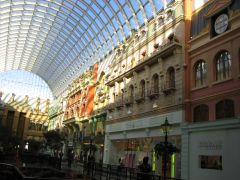
\includegraphics[width=.45\linewidth]{gfx/example_1}} \quad
    \subfloat[Pan ma signo.]
    {\label{fig:example-b}%
        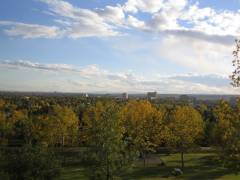
\includegraphics[width=.45\linewidth]{gfx/example_2}} \\
    \subfloat[Methodicamente o uno.]
    {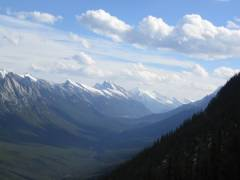
\includegraphics[width=.45\linewidth]{gfx/example_3}} \quad
    \subfloat[Titulo debitas.]
    {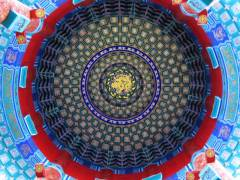
\includegraphics[width=.45\linewidth]{gfx/example_4}}
    \caption[Tu duo titulo debitas latente]{Tu duo titulo debitas
    latente. \ac{DRY}}\label{fig:example}
\end{figure}


%*****************************************
%*****************************************
%*****************************************
%*****************************************
%*****************************************

%\addtocontents{toc}{\protect\clearpage} % <--- just debug stuff, ignore
%\chapter{Espressioni regolari}
Le espressioni regolari sono un formalismo comunamente utilizzato per
definire linguaggi semplici.

\begin{theorem}
  La definizione induttiva di un espressione regolare su un alfabeto $A$:
  \paragraph{Base:}
  \begin{itemize}
    \item $0$ è un espressione regolare di $A$;
    \item $\lambda$ è un espressione regolare di $A$;
    \item per ogni $\sigma\in A$, $\sigma$ è un espressione regolare
      in $A$.
  \end{itemize}
  
  \paragraph{Passo induttivo:}
  \begin{itemize}
    \item se $e_1$ ed $e_2$ sono espressioni regolare di $A$,

      allora $e_1|e_2$ è un espressione regolare di $A$;
    \item se $e_1$ ed $e_2$ sono espressioni regolare di $A$,

      allora $e_1 e_2$ è un espressione regolare di $A$;
    \item se $e$ è un espressione regolare di $A$,

      allora $e^\star$ è un espressione regolarare di $A$.
  \end{itemize}
\end{theorem}

%\include{multiToC} % <--- just debug stuff, ignore for your documents
% ********************************************************************
% Backmatter
%*******************************************************
%\appendix
%\renewcommand{\thechapter}{\alph{chapter}}
%\cleardoublepage
%\part{Appendix}
%%********************************************************************
% Appendix
%*******************************************************
% If problems with the headers: get headings in appendix etc. right
%\markboth{\spacedlowsmallcaps{Appendix}}{\spacedlowsmallcaps{Appendix}}
\chapter{Appendix Test}
Lorem ipsum at nusquam appellantur his, ut eos erant homero
concludaturque. Albucius appellantur deterruisset id eam, vivendum
partiendo dissentiet ei ius. Vis melius facilisis ea, sea id convenire
referrentur, takimata adolescens ex duo. Ei harum argumentum per. Eam
vidit exerci appetere ad, ut vel zzril intellegam interpretaris.
\graffito{More dummy text.}

%Errem omnium ea per, pro congue populo ornatus cu, ex qui dicant
%nemore melius. No pri diam iriure euismod. Graecis eleifend
%appellantur quo id. Id corpora inimicus nam, facer nonummy ne pro,
%kasd repudiandae ei mei. Mea menandri mediocrem dissentiet cu, ex
%nominati imperdiet nec, sea odio duis vocent ei. Tempor everti
%appareat cu ius, ridens audiam an qui, aliquid admodum conceptam ne
%qui. Vis ea melius nostrum, mel alienum euripidis eu.

\section{Appendix Section Test}
Test: \autoref{tab:moreexample} (This reference should have a
lowercase, small caps \spacedlowsmallcaps{A} if the option
\texttt{floatperchapter} is activated, just as in the table itself
 $\rightarrow$ however, this does not work at the moment.)

\begin{table}[h]
    \myfloatalign
    \begin{tabularx}{\textwidth}{Xll} \toprule
        \tableheadline{labitur bonorum pri no} & \tableheadline{que vista}
        & \tableheadline{human} \\ \midrule
        fastidii ea ius & germano &  demonstratea \\
        suscipit instructior & titulo & personas \\
        %postulant quo & westeuropee & sanctificatec \\
        \midrule
        quaestio philosophia & facto & demonstrated \\
        %autem vulputate ex & parola & romanic \\
        %usu mucius iisque & studio & sanctificatef \\
        \bottomrule
    \end{tabularx}
    \caption[Autem usu id]{Autem usu id.}
    \label{tab:moreexample}
\end{table}

%Nulla fastidii ea ius, exerci suscipit instructior te nam, in ullum
%postulant quo. Congue quaestio philosophia his at, sea odio autem
%vulputate ex. Cu usu mucius iisque voluptua. Sit maiorum propriae at,
%ea cum primis intellegat. Hinc cotidieque reprehendunt eu nec. Autem
%timeam deleniti usu id, in nec nibh altera.




\section{Another Appendix Section Test}
Equidem detraxit cu nam, vix eu delenit periculis. Eos ut vero
constituto, no vidit propriae complectitur sea. Diceret nonummy in
has, no qui eligendi recteque consetetur. Mel eu dictas suscipiantur,
et sed placerat oporteat. At ipsum electram mei, ad aeque atomorum
mea. There is also a useless Pascal listing below: \autoref{lst:useless}.

\begin{lstlisting}[float=b,language=Pascal,frame=tb,caption={A floating example (\texttt{listings} manual)},label=lst:useless]
for i:=maxint downto 0 do
begin
{ do nothing }
end;
\end{lstlisting}

%Ei solet nemore consectetuer nam. Ad eam porro impetus, te choro omnes
%evertitur mel. Molestie conclusionemque vel at, no qui omittam
%expetenda efficiendi. Eu quo nobis offendit, verterem scriptorem ne
%vix.


%********************************************************************
% Other Stuff in the Back
%*******************************************************
%\cleardoublepage%********************************************************************
% Bibliography
%*******************************************************
% work-around to have small caps also here in the headline
% https://tex.stackexchange.com/questions/188126/wrong-header-in-bibliography-classicthesis
% Thanks to Enrico Gregorio
\defbibheading{bibintoc}[\bibname]{%
  \phantomsection
  \manualmark
  \markboth{\spacedlowsmallcaps{#1}}{\spacedlowsmallcaps{#1}}%
  \addtocontents{toc}{\protect\vspace{\beforebibskip}}%
  \addcontentsline{toc}{chapter}{\tocEntry{#1}}%
  \chapter*{#1}%
}
\printbibliography[heading=bibintoc]

% Old version, will be removed later
% work-around to have small caps also here in the headline
%\manualmark
%\markboth{\spacedlowsmallcaps{\bibname}}{\spacedlowsmallcaps{\bibname}} % work-around to have small caps also
%\phantomsection
%\refstepcounter{dummy}
%\addtocontents{toc}{\protect\vspace{\beforebibskip}} % to have the bib a bit from the rest in the toc
%\addcontentsline{toc}{chapter}{\tocEntry{\bibname}}
%\label{app:bibliography}
%\printbibliography

%\cleardoublepage%*******************************************************
% Declaration
%*******************************************************
\pdfbookmark[0]{Declaration}{declaration}
\chapter*{Declaration}
\thispagestyle{empty}
Put your declaration here.
\bigskip

\noindent\textit{\myLocation, \myTime}

\smallskip

\begin{flushright}
    \begin{tabular}{m{5cm}}
        \\ \hline
        \centering\myName \\
    \end{tabular}
\end{flushright}

%\cleardoublepage\pagestyle{empty}

\hfill

\vfill


\pdfbookmark[0]{Colophon}{colophon}
\section*{Colophon}
This document was typeset using the typographical look-and-feel \texttt{classicthesis} developed by Andr\'e Miede and Ivo Pletikosić.
The style was inspired by Robert Bringhurst's seminal book on typography ``\emph{The Elements of Typographic Style}''.
\texttt{classicthesis} is available for both \LaTeX\ and \mLyX:
\begin{center}
\url{https://bitbucket.org/amiede/classicthesis/}
\end{center}
Happy users of \texttt{classicthesis} usually send a real postcard to the author, a collection of postcards received so far is featured here:
\begin{center}
\url{http://postcards.miede.de/}
\end{center}
Thank you very much for your feedback and contribution.

\bigskip

\noindent\finalVersionString

%Hermann Zapf's \emph{Palatino} and \emph{Euler} type faces (Type~1 PostScript fonts \emph{URW
%Palladio L} and \emph{FPL}) are used. The ``typewriter'' text is typeset in \emph{Bera Mono},
%originally developed by Bitstream, Inc. as ``Bitstream Vera''. (Type~1 PostScript fonts were made
%available by Malte Rosenau and
%Ulrich Dirr.)

%\paragraph{note:} The custom size of the textblock was calculated
%using the directions given by Mr. Bringhurst (pages 26--29 and
%175/176). 10~pt Palatino needs  133.21~pt for the string
%``abcdefghijklmnopqrstuvwxyz''. This yields a good line length between
%24--26~pc (288--312~pt). Using a ``\emph{double square textblock}''
%with a 1:2 ratio this results in a textblock of 312:624~pt (which
%includes the headline in this design). A good alternative would be the
%``\emph{golden section textblock}'' with a ratio of 1:1.62, here
%312:505.44~pt. For comparison, \texttt{DIV9} of the \texttt{typearea}
%package results in a line length of 389~pt (32.4~pc), which is by far
%too long. However, this information will only be of interest for
%hardcore pseudo-typographers like me.%
%
%To make your own calculations, use the following commands and look up
%the corresponding lengths in the book:
%\begin{verbatim}
%    \settowidth{\abcd}{abcdefghijklmnopqrstuvwxyz}
%    \the\abcd\ % prints the value of the length
%\end{verbatim}
%Please see the file \texttt{classicthesis.sty} for some precalculated
%values for Palatino and Minion.
%
%    \settowidth{\abcd}{abcdefghijklmnopqrstuvwxyz}
%    \the\abcd\ % prints the value of the length

% ********************************************************************
% Game Over: Restore, Restart, or Quit?
%*******************************************************
\end{document}
% ********************************************************************
